\documentclass{proposalnsf}

\usepackage{array}
\usepackage{subfigure}
\usepackage{paralist}
\usepackage{enumitem}
\usepackage{listings}
\usepackage{color}
\usepackage{wrapfig}
\usepackage{stfloats}
\usepackage{comment}
\usepackage{palatino}
\usepackage{titlesec}

\usepackage{longtable}
\usepackage{latexsym}
\usepackage{amsmath, amsthm, amssymb}
\usepackage{amsfonts}
\usepackage[format=plain, font=small, labelfont=bf]{caption}
\usepackage{fancyhdr}
\usepackage[pdftex]{graphicx}
\usepackage[pdftex,
	    colorlinks=true, 	
	    pdfstartview=FitH,
	    linkcolor=blue,
	    citecolor=blue,
	    urlcolor=blue,
	    filecolor=black
	    ]{hyperref}
\usepackage{lscape}
\usepackage[T1]{fontenc}
\usepackage{floatrow}
\usepackage{pdfpages}
\usepackage{todonotes}
\usepackage{xspace}

 \titlespacing{\section}{0pt}{5pt}{3pt}
 \titlespacing{\subsection}{0pt}{3pt}{2pt}

%a few commands to highlight issues in the proposal (\TODO, \CHECK, \DummyText)
\RequirePackage{color}
\definecolor{RED}{rgb}{1,0,0}
\definecolor{BLUE}{rgb}{0,0,1}
\definecolor{White}{rgb}{1,1,1}

\providecommand{\CHECK}[1]{{\protect\color{blue} #1 (check) }}
\providecommand{\DummyText}[1]{{\protect\color{white} #1}}

\providecommand{\andrew}[1]{{\color{blue} Andrew: #1}}
\providecommand{\anote}[1]{{\color{red} Todo: #1}}

\newlength{\bibitemsep}\setlength{\bibitemsep}{.2\baselineskip plus .05\baselineskip minus .05\baselineskip}
\newlength{\bibparskip}\setlength{\bibparskip}{0pt}
\let\oldthebibliography\thebibliography
\renewcommand\thebibliography[1]{%
  \oldthebibliography{#1}%
  \setlength{\parskip}{\bibitemsep}%
  \setlength{\itemsep}{\bibparskip}%
}

\newcommand{\ignore}[1]{}

\newcommand{\degrees}{$\!\!$\char23$\!$}

\renewcommand{\refname}{\centerline{References cited}}

% this handles hanging indents for publications
\def\rrr#1\\{\par
\medskip\hbox{\vbox{\parindent=2em\hsize=6.12in
\hangindent=4em\hangafter=1#1}}}

\def\baselinestretch{1}

\setlength{\columnwidth}{\textwidth}

\usepackage{floatrow}
\floatsetup[table]{capposition=top}

\newcolumntype{L}[1]{>{\raggedright\let\newline\\\arraybackslash\hspace{0pt}}m{#1}}
\newcolumntype{C}[1]{>{\centering\let\newline\\\arraybackslash\hspace{0pt}}m{#1}}
\newcolumntype{R}[1]{>{\raggedleft\let\newline\\\arraybackslash\hspace{0pt}}m{#1}}

\usepackage{wrapfig}
\newcommand{\jc}[1]{{\footnotesize\color{blue}{[#1]}}}

\newcommand{\fillme}{{\bf XXX}~}
\newcommand{\eg}{{\it e.g.,}\xspace}
\newcommand{\ie}{{\it i.e.,}\xspace}
\newcommand{\etal}{{\it et.~al}\xspace}
\newcommand{\bigO}{\mathrm{O}}

\newcommand{\mypara}[1]{\smallskip\noindent{\bf {#1}:}~}
\newcommand{\myparatight}[1]{\vspace{0.03cm}\noindent{\bf {#1}:}~}
\newcommand{\myparaq}[1]{\smallskip\noindent{\bf {#1}?}~}


\newcounter{packednmbr}


\newenvironment{packedenumerate}{\begin{list}{\thepackednmbr.}{\usecounter{packednmbr}\setlength{\itemsep}{0.5pt}\addtolength{\labelwidth}{-4pt}\setlength{\leftmargin}{\labelwidth}\setlength{\listparindent}{\parindent}\setlength{\parsep}{1pt}\setlength{\topsep}{0pt}}}{\end{list}}


\newenvironment{packeditemize}{\begin{list}{$\bullet$}{\setlength{\itemsep}{0.5pt}\addtolength{\labelwidth}{-4pt}\setlength{\leftmargin}{\labelwidth}\setlength{\listparindent}{\parindent}\setlength{\parsep}{1pt}\setlength{\topsep}{0pt}}}{\end{list}}


\newenvironment{packedpackeditemize}{\begin{list}{$\bullet$}{\setlength{\itemsep}{0.5pt}\addtolength{\labelwidth}{-4pt}\setlength{\leftmargin}{\labelwidth}\setlength{\listparindent}{\parindent}\setlength{\parsep}{1pt}\setlength{\topsep}{0pt}}}{\end{list}}


\newenvironment{packedtrivlist}{\begin{list}{\setlength{\itemsep}{0.2pt}\addtolength{\labelwidth}{-4pt}\setlength{\leftmargin}{\labelwidth}\setlength{\listparindent}{\parindent}\setlength{\parsep}{1pt}\setlength{\topsep}{0pt}}}{\end{list}}


\newcommand{\tightcaption}[1]{\vspace{-0.12cm}\caption{{\em #1}}\vspace{-0.13cm}}
%\newcommand{\tightsection}[1]{\vspace{-0.02in}\section{#1}\vspace{-0.03cm}}
%\newcommand{\tightsubsection}[1]{\vspace{-0.02in}\subsection{#1}\vspace{-0.03cm}}
\newcommand{\tightsection}[1]{\vspace{-0.08cm}\section{#1}\vspace{-0.08cm}}
\newcommand{\tightsubsection}[1]{\vspace{-0.08cm}\subsection{#1}\vspace{-0.08cm}}
%\newcommand{\tightsection}[1]{\vspace{-0.0cm}\section{#1}\vspace{-0.0cm}}
%\newcommand{\tightsubsection}[1]{\vspace{-0.0cm}\subsection{#1}\vspace{-0.0cm}}
\newcommand{\tightsubsubsection}[1]{\vspace{-0.01in}\subsubsection{#1}\vspace{-0.01cm}}


\newcommand{\taskref}[1]{\textbf{Thrust~}\ref{#1}}
\newcommand{\subtaskref}[1]{\textbf{Task~}\ref{#1}}
\newcounter{tasknmbr}
\newcounter{tasklabel}

\newcounter{subtasknmbr}[tasknmbr]
\newcounter{subtasklabel}[tasklabel]

\renewcommand{\thesubtasklabel}{\textbf{\thetasknmbr.\thesubtasknmbr}}

\renewcommand{\thetasklabel}{\textbf{\thetasknmbr}}
\newenvironment{task}{
\begin{list}{\textbf{Task }\thetasklabel:~}{\usecounter{tasklabel}\stepcounter{tasknmbr}\setlength{\labelwidth}{0pt}\setlength{\labelsep}{0pt}\setlength{\leftmargin}{0in}\noindent \rule{\textwidth}{1pt}\vspace{-9pt} \rule{\textwidth}{1pt}\vspace{-9pt}\item \bf\em}}{\\[-7pt]\end{list}\vspace{-11pt}\noindent\rule{\textwidth}{1pt}\vspace{-9pt} \rule{\textwidth}{1pt}}

\newenvironment{subtask}{\vspace{-0.05cm}
\begin{list}{ \textbf{Task }\thesubtasklabel:~}{\usecounter{subtasklabel}\stepcounter{subtasknmbr}\setlength{\labelwidth}{0pt}\setlength{\labelsep}{0pt}\setlength{\leftmargin}{0in}\noindent \rule{\textwidth}{1pt}\vspace{-9pt}\item\em}}{\\[-7pt]\end{list} \vspace{-9pt}\noindent\rule{\textwidth}{1pt}}

%%%%%%%%%%%%%%%%%%%%%%%%%%%%%%%%%%%%%%%
%%%%% Document starts here

\begin{document}

%%%%%%%%%%%%%%%%%%%%%%%%%%%%%%%%%%%%%%%
% A - COVER SHEET: Produced by fastlane, type in information there.

%%%%%%%%%%%%%%%%%%%%%%%%%%%%%%%%%%%%%%%
% B - PROJECT SUMMARY
%{\bf \title} \\*[3mm]

%% {\bf Overview:} Each proposal must contain a summary of the proposed project not more than {\bf one page in length}. The Project
%% Summary consists of an overview, a statement on the intellectual merit of the proposed activity, and a statement
%% on the broader impacts of the proposed activity.

%% The overview includes a description of the activity that would result if the proposal were funded and a statement
%% of objectives and methods to be employed.  

%% The Project Summary should be written in the third person, informative to other persons working in
%% the same or related fields, and, insofar as possible, understandable to a scientifically or technically 
%% literate lay reader. It should not be an abstract of the proposal.
%% If the Project Summary contains special characters it may be uploaded as a Supplementary Document.
%% {\bf Project Summaries submitted as a PDF must be formatted with separate headings for the overview, statement on the
%% intellectual merit of the proposed activity, and statement on the broader impacts of the proposed activity}. Failure
%% to include these headings may result in the proposal being returned without review.
%% Additional instructions for preparation of the Project Summary are available in FastLane.\\
% \begin{center}
% %{\bf\large PROJECT DESCRIPTION} \\
% %\smallskip
% \vskip -1em
% {\sc  \small CRII: NeTS: Towards QoE-Aware Web Services}
% \end{center}

\begin{center}
{\bf\Large CRII: NeTS: Unleashing the Potential of QoE-Driven Web Backend} \\
\smallskip
\end{center}

\renewcommand{\thepage} {B--\arabic{page}}
%\newpage
%%!TEX root = main.tex

\vskip -.75em
\noindent {\bf Summary.~~} 
End-to-end QoE is the driving force behind Internet application ecosystem. The Internet application ecosystem consists of many subsystems, Cloud, ISP, CDNs, etc, and the way they work today follows an simple assumption that a subsystem should optimize all users using the same performance objective, if they look functionally the same (same service, business relationship, etc).

However, the Internet application ecosystem is essentially a faderated architecture. It has two profound implications: (1) For each end user, the perceived QoE can be affected by any subsystem along the way. (2) For each subsystem, it serves users whose QoE has different sensitivity to its quality.

This proposal is based on a simple insight: a subsystem should treat each user differently depending on how much its impact on the user's quality is, even if they look the same functionally.
This means that \jc{briefly describe why this is beneficial}

\noindent {\bf Intellectual Merit.~~}
This proposal applies this idea in the context of cloud services. 
\jc{what it means to cloud services? requests are going to be treated differently, etc} 
Specifically, this idea can be applied to many services inside a cloud. \jc{talk about more applications}
In this project, we plan to answer three key question:

First, how much potential benefit does this idea have?

Second, how to design a QoE-aware cloud scheduling/resource allocation mechanism?

Third, how to propogate QoE information from users to the cloud?

\noindent {\bf Broader Impacts.~~}


\noindent {\bf Keywords.~~} 



%%%%%%%%%%%%%%%%%%%%%%%%%%%%%%%%%%%%%%%
% C - TABLE OF CONTENTS: Automatically generated by fastlane.


%%%%%%%%%%%%%%%%%%%%%%%%%%%%%%%%%%%%%%%
% D - PROJECT DESCRIPTION

% reset page numbering to 1.  This is helpful, since the text can only
% be 15 pages (unless otherwise specified, see individual solicitations), 
% and reviewers will want to believe we've kept within those limits

%%  \newpage
%\tableofcontents
%\newpage

\pagenumbering{arabic}
\renewcommand{\thepage} {D--\arabic{page}}


%% The Project Description should provide a clear statement of the work to be undertaken and must include:
%% objectives for the period of the proposed work and expected significance; relation to longer-term goals of the PI's
%% project; and relation to the present state of knowledge in the field, to work in progress by the PI under other
%% support and to work in progress elsewhere.

%% The Project Description should outline the general plan of work, including the broad design of activities to be
%% undertaken, and, where appropriate, provide a clear description of experimental methods and procedures.
%% Proposers should address what they want to do, why they want to do it, how they plan to do it, how they will
%% know if they succeed, and what benefits could accrue if the project is successful. The project activities may be
%% based on previously established and/or innovative methods and approaches, but in either case must be well
%% justified. These issues apply to both the technical aspects of the proposal and the way in which the project may
%% make broader contributions.

%% The Project Description must contain, as a separate section within the narrative, a section labeled ``Broader
%% Impacts of the Proposed Work''. This section should provide a discussion of the broader impacts of the proposed
%% activities. Broader impacts may be accomplished through the research itself, through the activities that are
%% directly related to specific research projects, or through activities that are supported by, but are complementary to 
%% the project. NSF values the advancement of scientific knowledge and activities that contribute to the
%% achievement of societally relevant outcomes. Such outcomes include, but are not limited to: full
%% participation of women, persons with disabilities, and underrepresented minorities in science, technology, engineering, and
%% mathematics (STEM); improved STEM education and educator development at any level; increased public
%% scientific literacy and public engagement with science and technology; improved well-being of individuals in
%% society; development of a diverse,globally competitive STEM workforce; increased partnerships between
%% academia, industry, and others; improved national security; increased economic competitiveness of the United
%% States; and enhanced infrastructure for research and education.

%% Plans for data management and sharing of the products of research, including preservation, documentation, and
%% sharing of data, samples, physical collections, curriculum materials and other related research and education
%% products should be described in the Special Information and Supplementary Documentation section of the
%% proposal (see GPG Chapter II.C.2.j. for additional instructions for preparation of this section).

%\vspace{0.2in}

%\tableofcontents

%\newpage
%!TEX root = main.tex
%\vskip -.75em
%\mypara{Summary}
% \jc{yet another QoE improvement doesn't sound very exciting}
The ecosystem of web applications critically depends on maintaining desirable user-perceived QoE (quality of experience).
% QoE depends critically on web page loading time, 
Yet despite tremendous efforts,
%(\eg cutting tail latency via redundancy or pushing caches closer to end users), 
many users still suffer from suboptimal QoE.
%Unlike previous approaches such as cutting tails of response time or pushing caches closer to end users, 
This proposal introduces a new dimension for web QoE optimization that has been ignored by today's web backend: harnessing the {\em inherent heterogeneity} of how much impact backend delay has on the QoE of different users, even if they request the same type of application/service.
% {\bf QoE sensitivity to backend delay} across users. More importantly, such heterogeneity is prevalent even if the users request the same type of application/service.
%, \ie how sensitive a user's QoE is to the web backend delay.
For instance, a web request that has spent 50ms on wide-area networks before reaching the web server tends to be more sensitive to 10ms delay of web backend than a request that has already spent 500ms on the network does. 
Such discrepancy in QoE's sensitivity to backend delay has profound implications on how web backend should allocate its limited resources across requests.
In essence, web requests previously seen as indistinguishable by the backend can now be treated differently in such a way that favors the requests whose QoE is more sensitive to backend delay without hurting other requests' QoE. 
%We show early promising result that by making existing the web backend aware of QoE sensitivity, we could improve both QoE and resource efficiency than existing solutions.
To fully unleash these potentials, we propose to re-architect today's web backend by elevating the sensitivity of QoE to the backend delay as a key factor in the control logic of web backend.
% investigate new opportunities to improve QoE and save resources by making web services aware of QoE sensitivity (\eg better scheduling policies and replica selection policies) and 
We will provide a technical roadmap to quantify the potential improvement (better QoE and resource efficiency) of QoE-driven web backend in the wild and address the key challenges, including QoE-driven scheduling policies and replica selection policies, estimating the QoE sensitivity of each request, and addressing fairness issues.
% (1) We quantify its potential benefits in QoE and resource savings.
% (2) We propose novel algorithms for QoE-aware scheduling and resource allocation of web services. 
% (3) We present novel system designs and implement prototypes that make web services QoE-aware in practice.


% Thus, the goal of each subsystems in a large web service, such as web server or key-value store, should be to optimize the overall QoE of many users given limited resources. 
% A common approach to achieving this goal is for each subsystem to optimize some ``local'' performance metrics measured within its scope (\eg server-side delay) over all users, and the intuition is that if each subsystem follows the approach, it will optimize the overall QoE of users. 
% We argue, however, that this approach only achieves suboptimal QoE and can use more resources than necessary. 
% Our key observation is that {\em the impact of a subsystem's performance on a user's perceived QoE varies greatly among users} (modulo web page type, business relationship), so when sharing resources across users, each subsystem should take into account its impact on each user's QoE.
% One typical sources 
% This has profound implication on how web services should be optimized, and opens up many several new opportunities.


\section{Introduction}

% - QoE is important and our goal is to improve QoE for Web Services.
\noindent 
The fundamental challenge faced by large-scale web service providers (\eg Microsoft, Facebook, Google) is how to share resources of the web backend across users so as to optimize the user-perceived {\em QoE} (Quality of Experience). 
Web QoE has been shown to be critically dependent on web page loading time~\cite{??,??}.
Despite great amounts of efforts, ensuring desirable QoE is still an unsolved problem with \fillme\% users whose experience could have been improved from bad to good if the backend delay is zero~\cite{dqbarge}.

%Their business models, based on advertisement or subscription, are driven by user engagement, for which QoE is believed to play a vital role (among other factors such as content, user interfaces).

\mypara{Limitation of today's web backend}
Page load time, which we refer to as {\em end-to-end delay}, generally consists of three parts: client-side delay, wide-area network (WANs) delay, and backend delay.
%- Web services, like applications running in the cloud, have been basing their optimizations on the goal of improving server-side latency (sometimes the fraction of users meeting some fixed deadline)
%Because of the federated nature of Internet architecture, web service providers do not have full control over all types of delays.
%---to them, WANs and clients devices are largely blackboxes operated, not by the web services, but by ISPs, cellular carriers, and device vendors.
%(while web browsers and apps are developed by the web service providers, the client-side performance is largely decided by how OS share resources among multiple applications).
With web service providers only controlling the web backend, the performance metric they focus on optimizing is the 
%Thus, instead of optimizing for QoE directly, today's web services focus on reducing the 
%different requests have the same {\em QoE sensitivity to backend delay}
{\em backend delay}, under the assumption that a backend delay of $n$~ms has the {\em same} impact on any request.\footnote{Modulo the content-specific (\eg web page type) or user-specific (\eg free vs. premium subscription) factors.}
% That is, a backend delay of $n$~ms has the same effect on the QoE of any request.
For instance, they minimize the mean/tail backend delay or the fraction of requests whose backend delay exceeds some deadline (\eg 300ms).
%- This project takes a step back and asks a different question: does the latency have the same impact on user QoE? 
% In doing so, 
%all requests are optimized with the same objective function of backend response time; 
% an implicit assumption is that different requests have the same {\em QoE sensitivity to backend delay} (modulo content-/user-specific factors, such as web page type or subscription type, etc);
% that is, a backend delay of $n$~ms has the same effect on the QoE of different requests.

This proposal takes step back from this assumption, and ask {\em ``does each request really have the same sensitivity to backend delay?''}

%- The answer is no, which has profound impact on how web services should be built. [Give a simple example here.] In essence, this means giving each ``priority'', in terms of resources and scheduling, is cost-inefficient and suboptimal. [Give a simple example. resources wasted for users who are screwed already]
\mypara{Our insight} 
Our answer is {\em no}.  More importantly, even if the requests have no application-level differences (\eg web vs. video), such heterogeneous QoE sensitivity can still result from different non-backend delay (\eg wide-area network routing, client-side software)~\cite{timecard,dqbarge} across requests.
%Two observations contribute to this conclusion: the non-linear relationship between page load time and QoE~\cite{??} and the fact that the WAN/client delay varies among requests~\cite{timecard,dqbarge}, {\em the QoE sensitivity to backend delay varies among requests.}
For instance, a web request that has spent 50ms on wide-area networks before reaching the web server is more likely to be affected by 10ms delay of the web service than a request that has already spent 500ms on the network. 

The heterogeneous QoE sensitivity has profound implications for improving how web backend should allocate the limited resources among requests. 
By falsely assuming requests are equally sensitive to the backend delay, traditional web backend (Figure~\ref{fig:intro-overview}(a)) might waste precious resources (\eg wasting resources to optimize requests insensitive to the backend delay) and have suboptimal QoE (\eg spending inadequate resources on requests critically dependent on the backend delay). 
In contrast, the web backend should allocate resources smartly to each requests depending on their QoE sensitivity to the backend. 
On a message scheduling prototype, we found that such a QoE-driven scheduling policy can improve \fillme by \fillme\% over a baseline first-come-first-serve policy.
%\jc{bring up some concrete improvement numbers}
%\jc{need to highlight that this is not because application differents}

\begin{figure}[t]
	\centering
	\vspace{-0.5cm}
	\hspace{0.6cm}
	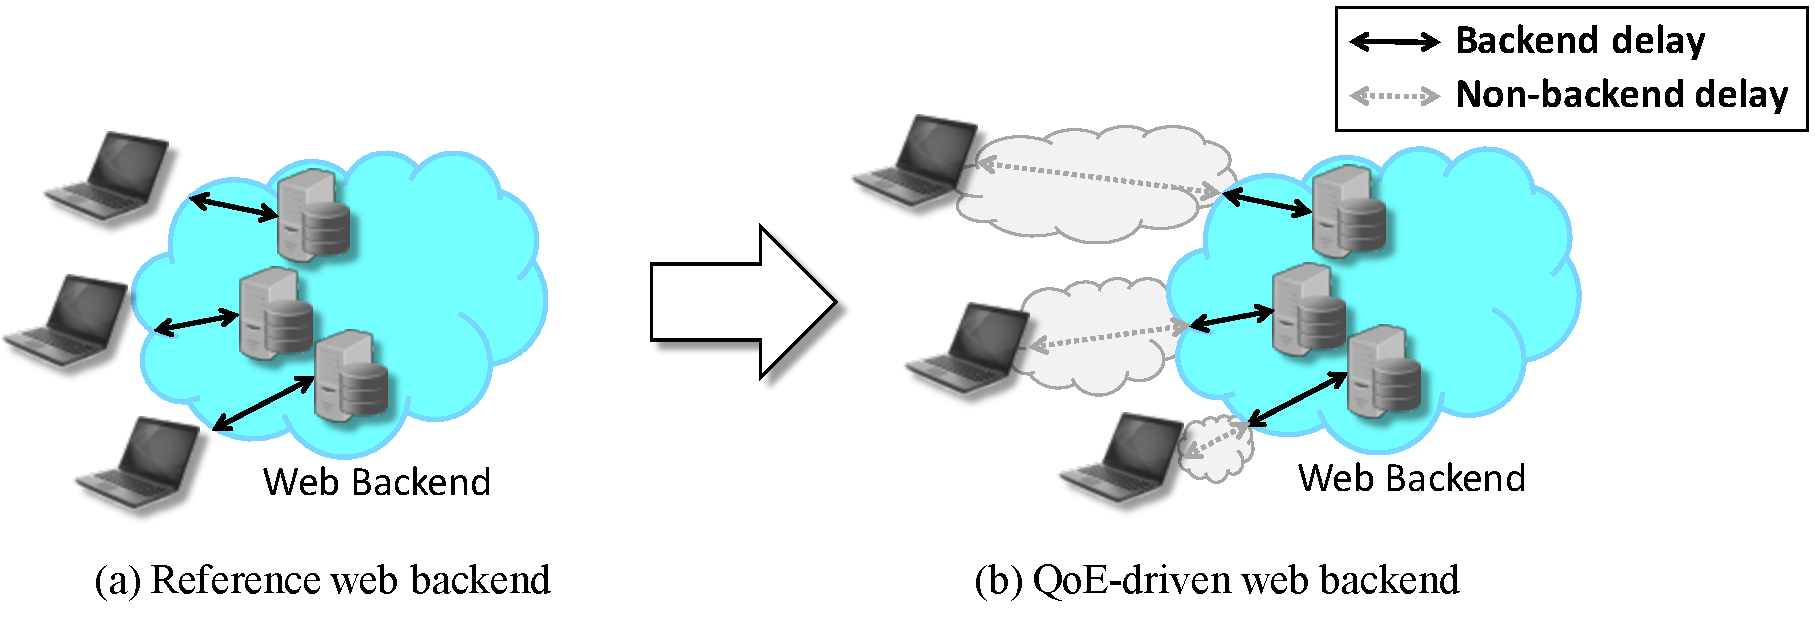
\includegraphics[width=0.9\textwidth]{figs/intro-overview.pdf}
	\vspace{-0.3cm}
	\caption{We propose to re-architect (a) the reference web backend which seeks to minimize the backend delays into (b) the QoE-driven web backend which seeks to minimize the impact of backend delay on user-perceived QoE.}
	\label{fig:intro-overview}
\end{figure}

%\jc{give a figure to contrast optimization of backend in-isolation vs. QoE-aware.}

%- Research goal: This project proposes that the web service backend should be aware of the QoE sensitivity. This effectively changes how one formulates the web service optimization problem.
\mypara{Research plan}
This proposal introduces ``QoE sensitivity'' as a new dimension for QoE optimization of web backends. 
Through developing novel algorithms and architectural components, we show that a {\bf QoE-driven web backend} (Figure~\ref{fig:intro-overview}(b)), which is aware of and exploits the differences of QoE sensitivity across requests, can substantially {\em improve the resource/QoE tradeoffs} of web service backend; \ie better QoE without using more resources, or saving resources without degrading QoE. 
% Note that being QoE sensitivity does not require expensive infrastructure changes (\eg adding hardware or changing software stack).
We divide the proposed research into four tasks.
%We use the following roadmap to thoroughly examine the benefits and challenges of QoE-sensitivity-aware web service backend.

\begin{packeditemize}
\item{\bf Quantifying potential benefits (Task \#1).}
We will design and carry out measurement studies to quantify the various improvements brought by QoE-driven web backend in the wild. We will provide a taxonomy of use cases of QoE-driven control in different aspects of today's web backend. We will also use large dataset from commercial web services to help understand opportunities in the actual traffic pattern in real world.

\item{\bf QoE-driven control algorithms (Task \#2).}
We will develop and build prototype of novel QoE-driven control policies for web backend, including resource allocation, message scheduling, and replica selection. Our design goals are (1) that the policies should balance near-optimal QoE and efficiency (minimal overhead of decision-making), and (2) that the implementation of these policies should be amenable to existing systems (\eg only control-plan changes).

\item{\bf QoE-driven backend architectural (Task \#3).}
We will develop new architectural component of web backend, including tracing infrastructure and QoE prediction models, to estimate the QoE sensitivity of requests in real-time. In the process, we will investigate the possibility of incremental deployment through reusing the existing tracing and telemetry infrastructure in large-scale web backends as much as possible.

\item{\bf Impact on QoE fairness (Task \#4).}
Finally, we will explore appropriate definitions of fairness to characterize the outcome of QoE-driven web backend. This would help us strike a desirable balance between QoE-driven optimization and QoE fairness. This would also help us recognize potential threads of other systems/users taking advantage of the QoE-driven policies of the backend.

\end{packeditemize}


%\jc{why these applications?}

%\jc{Common challenges! getting QoE sensitivity, fairness definition!}

\mypara{PI qualification}
The PI's expertise includes computer networking, Internet QoE, and data analytics systems.
He has published 11 peer-reviewed research papers (6 first-authored) in top-tier networking and system conferences (\ie SIGCOMM, NSDI, CoNEXT).
More importantly, the PI has a deep understanding of Internet QoE. His doctoral dissertation, titled ``Enabling Data-Driven Optimization of Quality of Experience in Internet Applications'', is among the first systematic studies to apply data-driven approach to improving Internet application QoE. The dissertation won the CMU SCS Doctoral Dissertation Award and was nominated for ACM Dissertation Award.
During his PhD and postdoctoral years, he has extensive collaborations with the industry, including Microsoft Research, Conviva Inc., and Google Research. These strong connections will help the proposed research to gain insights from the industry and provide viable path for deployment.


% \vspace{0.2cm}
% \noindent{\em Thrust \#1: How much potential benefit can we get?}

% \vspace{0.2cm}
% \noindent{\em Thrust \#2: How to re-architect web services to be QoE-aware?}

% \vspace{0.2cm}
% \noindent{\em Thrust \#3: How to propagate user-perceived QoE information?}

%- This project proposes to re-architect the web service backend by making it QoE-aware. Our roadmap has three steps.\\
%1. XXX\\
%2. YYY\\
%3. ZZZ



% \vspace{2cm}
% User-perceived quality of experience (QoE) is one of the driving forces behind the Internet ecosystem, which consists of {\em subsystems}, \eg datacenters, CDNs, cellular carriers, backbone networks, content providers, who share resources across users. 
% % End-to-end Quality of Experience (QoE) is the driving force behind today's Internet application ecosystem, which includes several subsystem
% % The Internet application ecosystem consists of many subsystems, Cloud, ISP, CDNs, etc, and 
% Thus, one fundamental question is {\em how to share resources across users in a way that optimizes their overall QoE?}
% The primary constraint is that these subsystems are {\em federated}: it is impractical to orchestrate a global optimization where they relinquish the control on how their resources are shared. 
% Instead, the conventional wisdom has been that each subsystem shares its resources among users in a way that optimizes the overall performance metrics within its limit and imposes no differentiation between users if they are ``functionally'' identical (\ie same service, business relationship, etc).

% In contrast, we are driven by a simple observation derived directly from the federated nature of the Internet ecosystem.
% In a subsystem, there is {\em a substantial heterogeneity} among its users with respect to how sensitive their QoE is to the performance of the subsystem, even if these users are functionally identical. 
% Thus, the right question to ask is {\em not} how a subsystem should optimize the overall performance among users; instead, it should minimize {\em overall impact on user-perceived QoE}, which requires treating users differently, rather than equally, depending on how much impact it has on the user's perceived QoE.

% In this proposal, we apply this idea to improving QoE of web services.

% \mypara{Research goals}

% \noindent {\bf Intellectual Merit.~~}
% This proposal applies this idea in the context of cloud services. 
% \jc{what it means to cloud services? requests are going to be treated differently, etc} 
% Specifically, this idea can be applied to many services inside a cloud. \jc{talk about more applications}
% In this project, we plan to answer three key question:

% First, how much potential benefit does this idea have?

% Second, how to design a QoE-aware cloud scheduling/resource allocation mechanism?

% Third, how to propogate QoE information from users to the cloud?

% \noindent {\bf Broader Impacts.~~}


% \noindent {\bf Keywords.~~} 



% QoE matters to everyone!

% \subsection{Missed Opportunities}
% \begin{itemize}

% \item Today's tenant: every user should be treated with the same performance goal. Implicit assumption is that the impact of a subsystem is the same on all users.

% \item However, the federated architecture means:\\
% 1. QoE can be affected by any subsystem\\
% 2. Each subsystem serves users with different QoE sensitivities.

% \item Fundamental mismatch: some users who are less sensitive to the subsystem get over-optimized, while others who are more sensitive to the subsystem get under-optimized.

% \item New approach: minimize the overall impact on QoE. 

% \end{itemize}

% \subsection{This proposal: Making Cloud QoE-Aware}
% \begin{itemize}

% \item How the cloud works today -- agnostic to QoE

% \item QoE curve

% \item Examples of how things can be done differently!

% \end{itemize}


% \subsection{Research Roadmap:}
% \begin{itemize}

% \item How much potential benefit does this idea have?

% \item How to design a QoE-aware cloud scheduling/resource allocation mechanism?

% \item How to propagate QoE information from users to the cloud?

% \end{itemize}


%!TEX root = main.tex

\section{Motivation and Framework}
In this section, we set up the context by introducing how today's web backends optimize QoE.
Then we show the key insight that there is a great heterogeneity in QoE's sensitivity to backend delay across requests, which inspires the proposed QoE-driven web backend.
%Then we give the empirical observation that there is great heterogeneity in the sensitivity of QoE to backend delay across requests, which inspires new opportunities to improve the QoE/resource tradeoffs of the web service backends without adding new resources. 
%Finally, we give a framework that contrasts today's approach with our proposed one.

\subsection{Today's approach}
% - Architecture of web service
%\mypara{A canonical architecture} 
\begin{wrapfigure}{r}{0.4\linewidth}
	\centering
	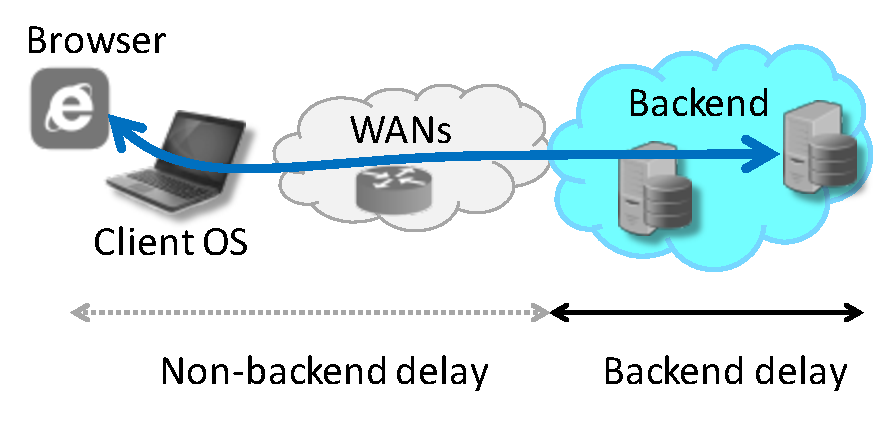
\includegraphics[width=1.0\textwidth]{figs/background.pdf}
	\caption{High-level architecture of web service and the workflow of a web request.}
	\label{fig:background}
\end{wrapfigure}
Figure~\ref{fig:background} depicts the high-level architecture of large-scale web services, and the typical workflow of a web request.
A web request (\eg loading of a front page) typically involves three components---client software, wide-area networks (WANs), and the backend---before the response is showed to the user.
The delay of each component contributes to the end-to-end delay and thus the user-perceived QoE (assuming the requested data is not cached locally by the client/ISP, etc). 
%In today's federated Internet architecture, the web service provider typically only has the control over the backend-induced delay. 
%Note that although client-side browsers/apps are developed by web service providers, the client-side delay is largely decided by how OS share resources among applications. 
A web backend can be viewed as solving a resource sharing problem: optimizing the performance of many requests using a limited amount of resources. 
With the web service providers only controlling the backend and the backend-induced delay\footnote{Although client-side browsers/apps are developed by web service providers, the client-side delay is largely decided by how OS share resources among applications.}, they seek to minimize the backend delay. 


% - Optimization metrics of each components: not QoE specific!
%\mypara{Today's approach}

To some extent, today's  backend systems assume (though often made implicitly) that the backend delay has the {\em same effect} on any request; \eg a delay of 20ms reading data from a database degrades the QoE by the same amount for any request. 
Under this assumption, it is sensible to measure performance by mean or percentiles (\eg 99$^\textrm{th}$ percentile) of backend delay or percentage of requests whose delays exceed some threshold (\eg service-level agreement).
Here, we only consider requests of the same application-level type, \eg content genre, user subscription type.

\subsection{Key insight: Heterogeneity of QoE sensitivity}
%\jc{throw in some concrete improvement numbers}

\begin{wrapfigure}{r}{0.45\linewidth}
	\centering
	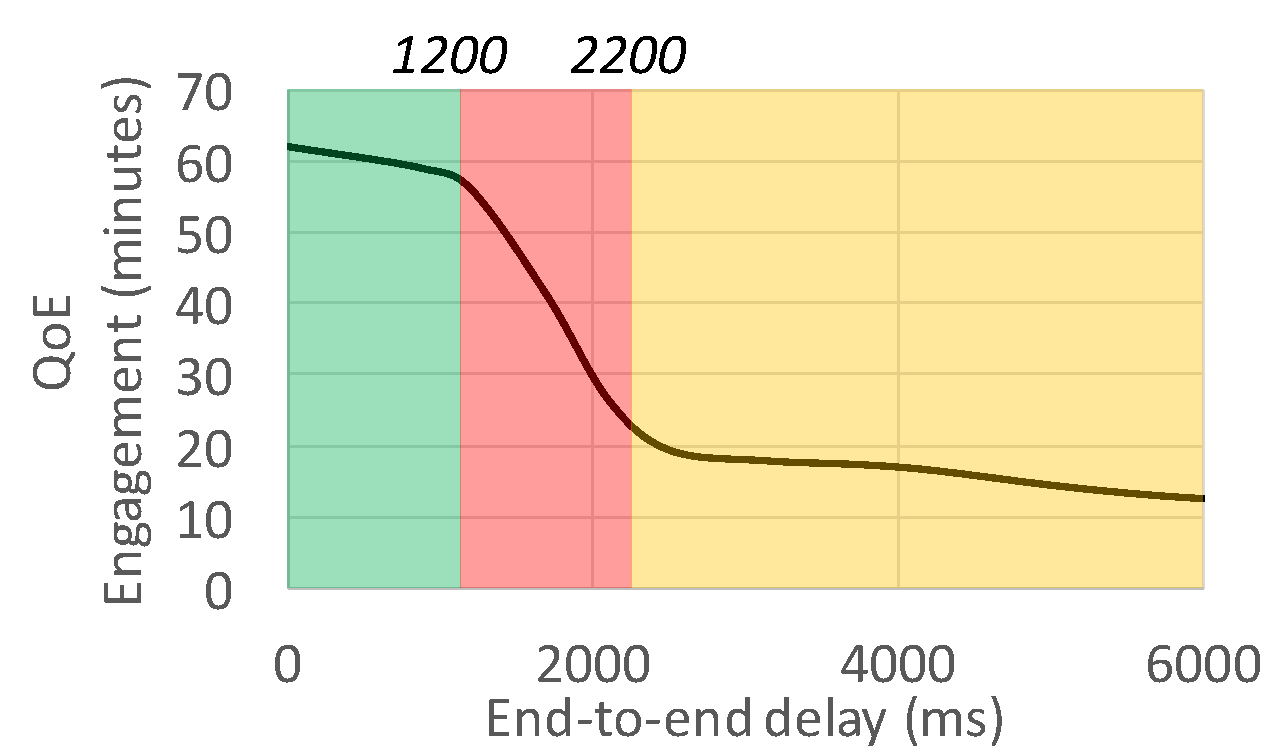
\includegraphics[width=0.95\textwidth]{figs/qoe-curve.pdf}
	\caption{QoE curve: relationship between QoE and the end-to-end delay of a request.}
	\label{fig:qoe-curve}
\end{wrapfigure}
Contrary to the assumption of backend delay having equal impact on QoE for any request, our key observation is that 
{\em the sensitivity of QoE to the backend delay varies across requests.}
%Our key observation is that the impact of backend delay on the QoE of a request actually depends on how much non-backend delay (Figure~\ref{fig:background}) the request experiences, including the client-induced and WAN-induced delays. 
%In other words, {\em the sensitivity of QoE to the backend delay varies across requests.} 
%\mypara{Why QoE sensitivity varies}
Figure~\ref{fig:qoe-curve} illustrates this observation using a dataset of \fillme web requests. The dataset includes all requests to one of the Alexa top-50 pages~\cite{??} over a span of 24 hours from \fillme countries, thus representing a decent spatio-temporal coverage of users while avoiding the impact of content-specific factors on QoE. 
The figure shows the relationship between QoE and the end-to-end delay of a request, which we refer to as the {\em QoE curve}.
%It is based on \fillme requests to a particular page (\fillme), thus avoiding the impact of content on QoE. 
For each request, we define QoE by user engagement (as in~\cite{??,??}): the duration of the user staying on the web page and all subsequent pages linked from the page. 
The end-to-end delay is calculated by subtracting when the page is completely loaded by when the request is issued. 

The important feature of curve is that its non-linear (sigmoid-like) shape.
Thus, the same amount of backend delay (\ie increase of end-to-end delay) will affect the QoE differently, depending on the position on the curve.
It can be intuitively explained as following.
Users are not sensitive to a small backend delay either when the overall delay is so short that it is imperceptible, or when it is too long that the user has mostly tired of waiting, but when the delay is in between can some change make a significant difference. 
Take the QoE curve in Figure~\ref{fig:qoe-curve} as an example: QoE is much more sensitive to the backend delay when the total delay is between roughly 1200ms and 2200ms than it is below or above that range.\footnote{This curve may vary with the nature of the web sites and the requests (\eg QoE in general is less sensitive to delay when the user really needs to see the content of the page than when the website tries to entice users to do something), yet the sigmoid-like shape remains.}
%Secondly, we observe that the non-backend delays (client- and WAN-induced delays) of the requests are not concentrated in certain segment of the curve; rather, they spread out over the curve.
%In our dataset, we found \fillme\% requests have non-backend delay are below 1200ms, \fillme\% between 1200ms and 2200ms, and \fillme\% above 2200ms. 
%Combining this observation with the non-linear relationship between delay and QoE, we see that the sensitivity of QoE to the backend delay varies among requests. 

%\myparaq{What is new}


%We are not the first to observe the heterogeneity in non-backend delay across requests~\cite{timeciard,dqbarge} and the non-linear delay-QoE relationship~\cite{d3tcp, mun chiang's work}---in fact, the assumption that application flows have deadline utility function can be viewed as a simplification of the non-linear delay-QoE relationship.
%What is new is their corollary that requests have different QoE sensitivity to backend delay, which, as we will see next, has a profound implication on QoE optimization.
%how resource consumption and QoE optimization should be balanced.
%if the backend can add a total backend delay of $\delta=\delta_a+\delta_b$ to the two requests ($A$ gets $\delta_a$ and $B$ gets $\delta_b$), traditional methods will give both $A$ and $B$ a delay of $\delta/2$, whereas better QoE can be achieved by letting $\delta_a<\delta_b$. 
%We will give more concrete examles in \S\ref{sec:design}.

\subsection{Motivating example}
\label{subsec:example}
Indeed, we are not the first to observe the heterogeneous impact of backend delay on QoE~\cite{timeciard,dqbarge,??,??}, but few work has systematically applied this observation to the problem of resource allocation across requests in the context of web backend.
At a high level, rathter than treating all requests as having equal sensitivity to the same amount of backend resources, the backend should instead allocate idle resources to requests that are more sensitive to backend delay.
Here we use a simple and yet realistic simulation to illustrate the benefits of QoE-driven resource allocation.
%, and then explain how it differs to traditional resource allocation approaches.

%To see it in action, suppose that request $A$ with non-backend delay $x_a$ is more sensitive to the backend delay (the red area of Figure~\ref{fig:qoe-curve}) than request $B$ with non-backend delay $x_b$ (the green or yellow area of Figure~\ref{fig:qoe-curve}). Now, if the backend resource allocation is such that one of them will get a backend delay of $\delta_1$ and the other one $\delta_2$, $\delta_1>\delta_2$. A QoE-agnostic method may make a random decision (\eg 50\% probability $A$ will get an end-to-end delay of $x_a+\delta_1$), but a QoE-driven method should instead assign the smaller backend delay $\delta_2$ to $A$, because $A$ is more sensitive to backend delay.

%Here, we run a simple simulation to quantify this improvement using the QoE curve shown in Figure~\ref{fig:qoe-curve}. 
Suppose we have 1000 requests whose QoE curve is shown in Figure~\ref{fig:qoe-curve}, and their non-backend delays are such that 29.8\% draw uniformly randomly from 0-1200ms (green part), 41.5\% from 1200-2200ms (red part), and 28.7\% from 2200ms to 6000ms (yellow part). This distribution matches the non-backend distribution in the dataset of Figure~\ref{fig:qoe-curve}.
We pre-generated 1000 backend delay values uniformly between 100-300ms. 
First, we consider a baseline that picks a random backend delay from the 1000 values (without replacement) for each request. The average QoE values is 37.6 (duration in minutes spent on the website).
Now, we imagine a QoE-driven policy that assigns the lowest 41.5\% backend delay values to the request between 1200-2200ms, and the rest requests gets randomly assigned delay values (without replacement). 
The average QoE now is 38.5, almost one-minute longer than the traditional method. In the QoE of the red part (QoE sensitive users), the improvement is almost 2.2 minutes longer than the traditional method!
Note that these improvements could potentially be achieved by simply prioritizing requests differently, without adding new resources or changing the underlying resource allocation mechanism (more on this in \S\ref{sec:design}).

It is important to note that such outcome will not naturally emerge from traditional methods that assign equal amount of resources to requests.
Even resource allocation policies that might naturally prioritize some requests over others (\eg in deadline-driven congestion control~\cite{??}, a few randomly picked flows might be delayed so that most flows can meet the flow completion deadline), such prioritization is still under the assumption that requests have the same sensitivity to the backend delay.


%\jc{add inefficiency of non-QoE-aware approaches: 
%resources wasted, packing qoe-sensitive users with non-sensitive users}

\subsection{Framework}
\label{subsec:framework}
Next we present a high-level framework (Figure~\ref{fig:framework}) of transforming today's web service backend with QoE-aware optimization.
Our design takes a pragmatic stance and confine ourselves to the minimal necessary changes on today's web backend.

\begin{wrapfigure}{r}{0.45\linewidth}
	\centering
	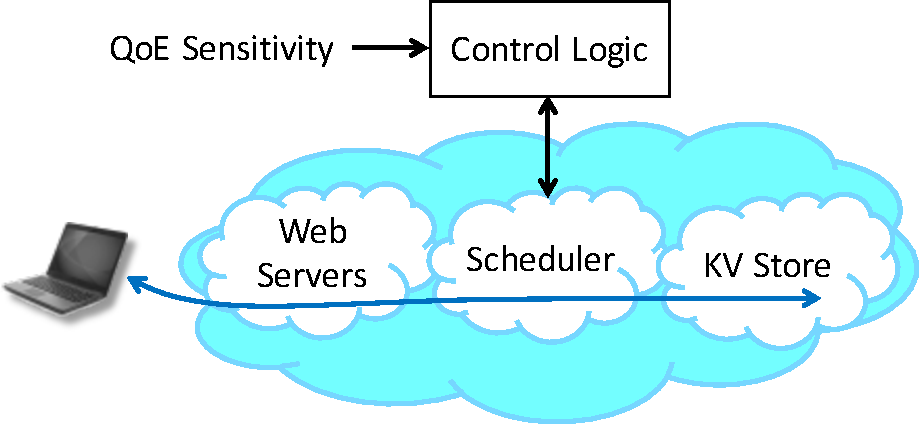
\includegraphics[width=1.0\textwidth]{figs/framework.pdf}
	\caption{QoE-driven web backend framework.}
	\label{fig:framework}
\end{wrapfigure}
We envision each individual subsystem (\eg web servers, messaging brokers, key-value stores, etc) has a resource-allocation control logic (\eg scheduling, queuing logic, replica selection logic, congestion control).
In a QoE-driven web backend, the control logic of a subsystem takes in as part of its input the QoE sensitivity of any incoming request---an estimate on its non-backend and the corresponding position on the QoE-latency curve. 
We will discuss how this information could be obtained in  \S\ref{sec:arch}.
%We envision different ways in which this information would be provided; \eg through a service that predicts the non-backend delay of a new request by profiling the non-backend delay of similar history requests, or adding a field in the request for any subsystem to tag the time it leaves each subsystem. (More discussion in \S\ref{sec:arch}.)

Then, the control logic needs to be updated to utilize the discrepancy of QoE sensitivity.
The contrast between the proposed QoE-aware control logic and traditional control logic can be explained as following: 
For each request $r$ in a set of requests $R$, let $t_{r}^{(nonbackend)}$ denote the non-backend delay, and $t_{r}^{(backend)}$ the backend delay, and $Q(t)$ the QoE of the total backend and non-backend delay $t$.
Traditional logic seeks to minimize average backend delay, \ie
\begin{align}
& \min \sum_{r\in R} t_{r}^{(backend)} \label{eq:old}
\end{align}
whereas, QoE-aware logic seeks to minimize average degradation of QoE, \ie
\begin{align}
& \min \sum_{r\in R} Q\left(t_{r}^{(nonbackend)}\right)-Q\left(t_{r}^{(nonbackend)}+t_{r}^{(backend)}\right) \label{eq:new}
\end{align}

Although ideally, we would like the multiple subsystems of the web backend to jointly optimize the backend delay of each request, there is little support of cross-subsystem orchestration across these subsystems, despite that they are typically owned by the same corporate/organization. So in  the proposed resolution, we only consider making individual subsystems aware of QoE sensitivity. Cross subsystem QoE optimization will be briefly discuss in \S\ref{sec:design}.


% shows a conceptual view of a QoE-aware web service backend. 
%A typical web service backend has multiple subsystems, \eg messaging system, distributed database, inter-datacenter networks, and any delay caused by any subsystem will contribute to the backend delay of a request.
%Although these subsystems are owned by the same organization, today there is little orchestration across these subsystems to jointly optimize for each request. 
%It is beyond our scope to discuss the cost of separating these subsystems. 
%
%
%
%This proposal takes a pragmatic stance. 
%We optimize each individual subsystem by proposing minimal necessary changes in its existing ``control logic''.
%A control logic can be implemented in different forms---\eg scheduling logic, resource allocation logic, congestion control sending rate, but it essentially share the limited resource among many requests.
%\begin{packeditemize}
%    \item The control logic of a QoE-aware subsystem takes in as part of its input the QoE sensitivity of any incoming request---an estimate on its non-backend and the corresponding position on the QoE-latency curve. 
%    We envision different ways in which this information would be provided; \eg through a service that predicts the non-backend delay of a new request by profiling the non-backend delay of similar history requests, or adding a field in the request for any subsystem to tag the time it leaves each subsystem. (More discussion in \S\ref{sec:arch}.)
%    \item Then, the control logic needs to be updated so that it can utilize the discrepancy of QoE sensitivity among requests to strike better QoE/resource tradeoffs (\ie the benefits we discussed in \S\ref{subsec:opportunities}).
%    The contrast between the proposed QoE-aware control logic and traditional control logic can be explained as following: 
%    For each request $r$ in a set of requests $R$, let $t_{r}^{(nb)}$ denote the non-backend delay, and $t_{r}^{(b)}$ the backend delay, and $Q(t)$ the QoE of the total backend and non-backend delay $t$.
%    Traditional logic seeks to minimize average backend delay, \ie
%    \begin{align}
%        & \min \sum_{r\in R} t_{r}^{(backend)} \label{eq:old}
%    \end{align}
%    whereas, QoE-aware logic seeks to minimize average degradation of QoE, \ie
%    \begin{align}
%        & \min \sum_{r\in R} Q\left(t_{r}^{(nonbackend)}\right)-Q\left(t_{r}^{(nonbackend)}+t_{r}^{(backend)}\right) \label{eq:new}
%    \end{align}
%\end{packeditemize}




\section{Quantifying Potential Benefits in the Wild}
\begin{task}
We will carry out measurement studies to quantify the benefits---in QoE and resource-efficiency---of a QoE-aware web service backend.
\end{task}

%The heterogeneity of QoE sensitivity across requests opens up many new opportunities to strike better resource/QoE tradoffs. 
In this section, we outline a measurement study to characterize and quantify the potential performance advantages of QoE-driven web backend in the wild.

%a taxonomy to categorize various possibilities of using the heterogeneous QoE sensitivity to improve the web service backend.%, and show simple-yet-realistic motivating examples to highlight two concrete use cases.

\subsection{Exploring the space of QoE-driven benefits}
\label{subsec:benefits}

\mypara{Performance metrics that can benefit}
As the first step, we categorize performance metrics along which a QoE-driven backend outperforms today's backend systems.
\begin{packeditemize}
\item{\em Improving QoE without adding more resources:} 
First and foremost, a QoE-driven backend can achieve better QoE than a traditional one by allocating resources in a way that more explicitly optimizes the total QoE. 
The basic idea is to switch resources from requests that are insensitive to backend delay to those that are sensitive.
We have seen an example of this in \S\ref{subsec:example}.
%In contrast to today's web backends which focus on the mean (or percentiles) of backend delay, we argue that they should instead {\em minimize the impact of backend delay on QoE}, so more resources (\eg higher priority) should be given to requests whose QoE is more sensitive to the backend delay. 

\item{\em Saving resources without hurting QoE:}
Similarly, one can reduce resource consumption (and thus save energy) by spending less resources to those requests of lower sensitivity to the backend delay. For instance, this can be done by allocating less CPU cycles or memory to servers that serve these requests or sending them to servers with higher load.

\item{\em Mitigating the impact of performance outliers:} 
Web backends are susceptible to performance outliers---excessively long delay due to \eg server garbage collections. 
Rather than trimming the outliers, we take a different approach---reducing the {\em degradation} of QoE caused by outliers.
For instance, we can profile the performance of servers, and assign only requests with less QoE sensitivity to the those likely to have outliers~\cite{ganesh's trimming}. 
    
\item{\em Cost-efficient explorations:}
To cope with dynamic resource availability and network conditions, web backends need to monitor the performance of multiple decisions (\eg edge clusters) by sending some random requests to use suboptimal decisions or injecting active probing traffic, neither of which is ideal.
We take a different approach---we can use the requests that are less sensitive to backend delay to probe the suboptimal decisions, as long as the resulting QoE degradation is below the overall QoE improvement.
\end{packeditemize}

%does not exceed the QoE gain of sending a request of high QoE sensitivity to the optimal decision.
% This way, we can maintain visibility with less impact on QoE.
%\end{packeditemize}

Note that at first glance, these optimizations may seem unfair, but as we will discuss in \S\ref{sec:arch}, this can still be fair in the sense that each request gets an equal treatment (degradation) on the QoE.
Importantly, these benefits can be realized without expensive adding more hardware or changing software stack, and can be done incrementally (they have no inter-dependency).

\mypara{Use cases that can benefit}
The improvements along performance metrics can manifest themselves in different use cases in web backend (Figure~\ref{fig:framework}): 
\begin{packeditemize}

\item {\em Resource allocation:} 
Better allocation of resources, such as CPU, RAM, network bandwidth, that are shared by multiple concurrent requests. 

\item {\em Scheduling:}
Scheduling of requests shares resource (\eg slot in a queue) along temporal dimension.
Uses of scheduling include message broker, job scheduler, etc.

\item {\em Replica selection:}
Performance of replicas depends critically on how requests are assigned.
Uses of replica selections include selections of web servers, nodes of a distributed key-value store (or database), partition-aggregating nodes.

\end{packeditemize}

Besides web services, it is worth noting that video streaming providers can use similar ideas to improve video QoE. For instance, the video servers can allocate more resources (\eg bandwidth, I/O cycles) to video sessions whose buffer is about to be empty (which means the QoE is more sensitive) than to those whose buffer is long enough.

\subsection{What-if analysis of potential improvement}

Next, we examine that under what conditions can QoE-driven web backend significantly outperforms traditional ones. 
The simple example in \S\ref{subsec:example} illustrates that the improvement of QoE-driven depend on three factors.

Firstly, the workload must be a mix of requests whose QoE is sensitive to the backend and those whose QoE is insensitive. 
Take Figure~\ref{fig:qoe-curve} as an example, if all requests are in the red region (sensitive to backend delay) or all in the yellow and green regions (insensitive to backend delay), we will see  little performance improvement over the baseline, because the backend delay will have the same effect on QoE. 
The improvement will be significant when sensitive requests and insensitive requests are both present, as in the example of \S\ref{subsec:example}.
%, we found 41.5\% requests have QoE that is sensitive to the backend delay (red region between 1200ms and 2200ms), and the rest (29.8\% in the green region and 28.7\% in the yellow region) have QoE that is not as sensitive to the backend delay. 

Secondly, requests should have different backend delay, which distributed systems naturally have for a number of reasons, \eg jobs in a queue will naturally have different waiting time, or replicas will naturally have different performance since they have different load.

Last but not least, the backend delay must not be too large or small a portion of the end-to-end delay. Too large, the end-to-end delay will be dominated by the backend delay, making all requests similarly sensitive to the backend delay. Too small, the backend delay will only have a very marginal impact on the end-to-end delay and QoE. 
Prior measurement studies (\eg~\cite{dqbarge,mysterymachine,timecard}) have shown that the backend delay constitute is a non-trivial yet not dominant portion of the end-to-end delay.


\subsection{Proposed research}
%- Quantifying the QoE-delay curve in the wild
We propose to run measurement studies and trace-driven analysis to characterize the QoE-driven opportunities along three aspects.
First, we will perform a mix of user studies and trace-driven analysis to create QoE curve for various web sites (\eg Alexa top sites) and different users (\eg various devices, demographic areas) to confirm that the impact of backend delay on QoE does varies.
%- Quantifying the heterogeneity of QoE sensitivity
Second, we will work with large content providers to gain insights as to whether real-world workload is a mix of sensitive and insensitive requests and the backend delay is variable. 
Based on our discussion with Microsoft, it is expected that this task can use real-world data.
%- Impact of QoE-aware logic on QoE (maybe delay is too small to be noticed anyway)
Finally, to efficiently explore the whole space of advantages (performance metrics and use cases presented in \S\ref{subsec:benefits}), we plan to scale the evaluation by developing a trace-driven simulator that uses real trace to estimate the potential improvement without actually deploying QoE-driven web backend.




\section{Designing QoE-Aware Web Service Backend}
\label{sec:design}

\begin{task}
We will develop new control policies (including scheduling, replica selection) that leverage the heterogeneity of QoE sensitivity across requests to improve the QoE/resource tradeoffs.
\end{task}

In this task, we will focus on the control logic of scheduling and replica selection as the locus of QoE-driven optimization. 
We start with why traditional scheduling and replica selection policies are insufficient.
Then we highlight technical challenges behind the QoE-driven control logic.

\subsection{Why are new policies needed?}


\mypara{Message scheduling}
Scheduling of messages~\cite{??} and jobs~\cite{??} in queues is pervasively used in the web backend. 
For instance, a message broker is a typical queuing system that provides subscriber/publisher services between two subsystems (\eg web servers and database stores). 

% - fifo and etc don't work
\begin{wrapfigure}{r}{0.48\linewidth}
	\centering
	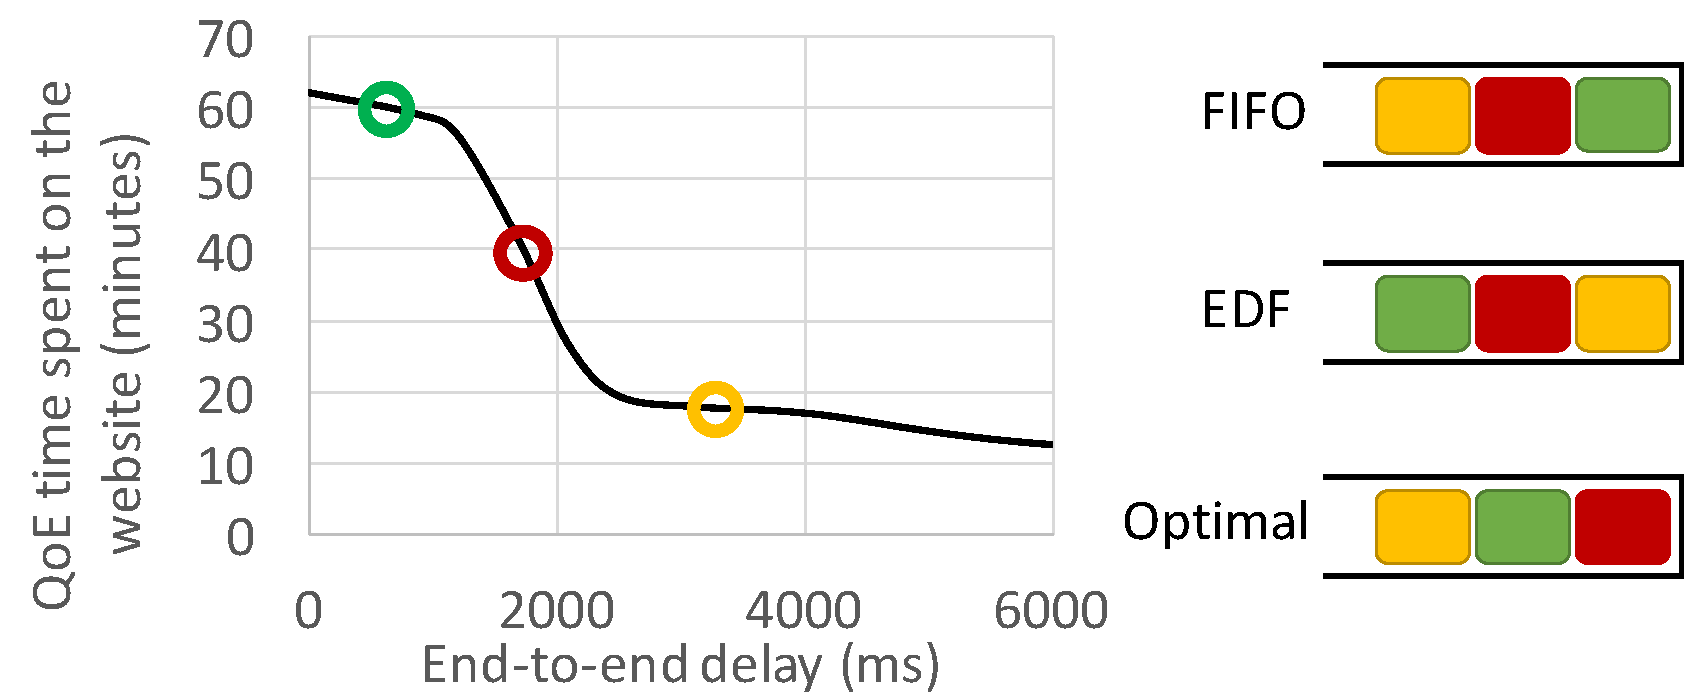
\includegraphics[width=1.0\textwidth]{figs/scheduling.pdf}
	\caption{The outcomes of different scheduling policies (right) applied on the three requests with different positions on the QoE curve (left).}
	\label{fig:scheduling}
\end{wrapfigure}
Figure~\ref{fig:scheduling} illustrates the need for a new policy for QoE-driven scheduling. 
We consider three requests in a queue, which are identical except their non-queuing delays (shown on the left-hand side of Figure~\ref{fig:scheduling}).
We compare three policies: 
(1) FIFO, which is the default policy for equal-priority requests.
(2) Earliest-Deadline-First (EDF), which give the requests with longer non-queuing delay higher priority (\ie closer to the deadline), and 
(3) the optimal scheduling policy (Optimal) that maximizes average QoE.
Here, the end-to-end of a request is the sum of the backend delay (\ie the number of jobs ahead of it times the per-request processing delay) and the non-backend delay.
Figure~\ref{fig:scheduling}  shows the outcome of running each policy. 
Because FIFO and EDF are agnostic to the sensitivity of QoE (\ie the slope of each request on the QoE curve), they are not aware that the most sensitive request is the red one.
In contrast, the Optimal policy is able to identify and prioritize the red request one over the others.
%OPT also outperforms EDF with various deadlines, even though it somehow takes the non-queuing delay into account (by imposing a deadline on the total of queuing and non-queuing delay).
%This is because how close a request's non-queuing delay is to the deadline is {\em still} agnostic to the sensitivity of QoE to the queuing delay. 
%Remember in Figure~\ref{fig:qoe-curve}, the QoE sensitivity does not grow monotonically to the non-backenc(queuing) delay. 

\mypara{Web server replica selection}
% - example of tails
Large-scale distributed systems are susceptible to {\em performance outliers}.
% on some replicas---\eg exceptionally long processing time on some requests due to CPU contention, software garbege collection, etc. 
Despite much effort to eliminate performance outliers, they are still prevalent, resulting in bad tail (\eg 99$^\textrm{th}$ percentile) performance even if the mean/median performance is good.
%Our first idea is that rather than cutting the performance outliers, we show that QoE-aware replica selection algorithm can {\em contain} the negative impact of performance outliers on user-perceived QoE.


\begin{wrapfigure}{r}{0.5\linewidth}
	\centering
	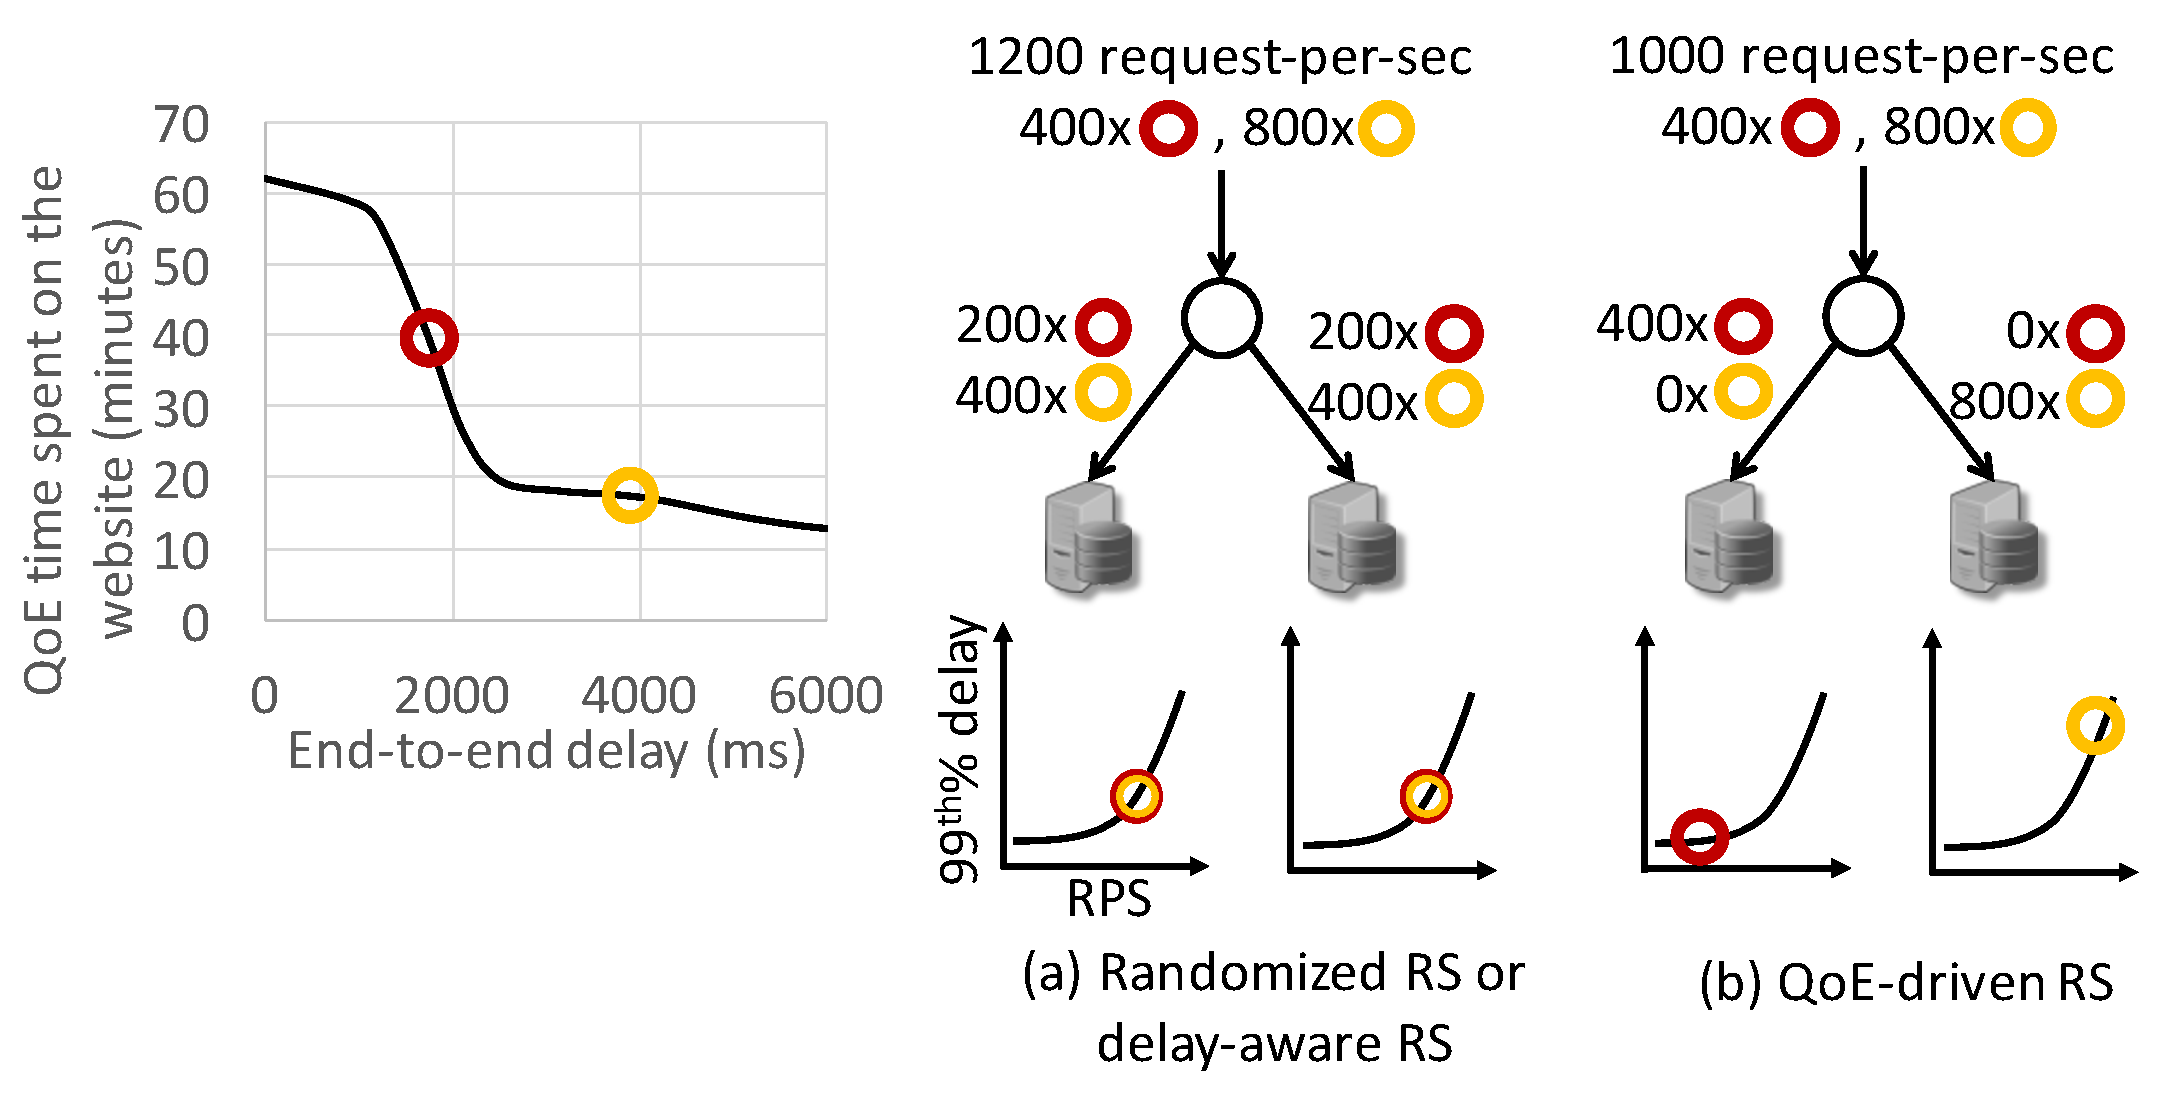
\includegraphics[width=1\textwidth]{figs/replica.pdf}
	\caption{A simple example showing the outcomes of different replica selection policies.}
	\label{fig:replica}
\end{wrapfigure}
%Consider a system with two replicas, as in Figure~\ref{??}. 
Figure~\ref{fig:replica} illustrates an example where a QoE-driven replica selection policy can contain the negative impact of performance outliers on user-perceived QoE, but a traditional load-balancing policy is not able to do so.
Both replicas have the same load-performance profile: as load (number of requests received per second) goes up, the 99$^\textrm{th}$ percentile delay increases sharply. We assume that the mean delay remains the same. 
This illustrative setting is simplified but in consistent with the load-performance profile in real datacenters~\cite{??}.
Suppose that the workload is 1200 requests per second, that the requests have same QoE curve, and their non-backend delays follow the distribution show in the figure.
We compare two traditional replica selection policies---a randomized policy that strives to put even load, a latency-aware policy~\cite{c3,cassandra,etc} that optimizes for Eq.~\ref{eq:old}---with a QoE-driven policy that optimizes for Eq.~\ref{eq:new}.
The optimal solution achieves better tail QoE than both baselines. 
Both load balancing policy and latency-aware put even load to the replicas, which make both equally overloaded, causing long tail delay and bad tail QoE.
In contrast, the optimal policy diliberately puts more requests on one than another, but does so by letting QoE-sensitive requests use the lighter-loaded replica and letting QoE-insensitive requests use the slightly more loaded replica. 

In short, we see that, in both scheduling and replica selection, traditional QoE-agnostic policies are fundamentally unable to achieve the same performance as optimal QoE-driven policies. However, implementing an optimal  QoE-driven policy in practice is challenging.

\subsection{Why challenging?}

In general, a QoE driven policy should meet two requirements: {\em near-optimal} (\ie achieve QoE close to the optimal scheduling outcomes) and {\em efficient} (\ie constant decision time on each incoming request).
To see why meeting both requirements is challenging, let us take scheduling as an example and consider two baselines.
%The new QoE-aware scheduling policy should be {\em near optimal} (\ie achieve QoE close to the optimal scheduling outcomes) and {\em efficient} (\ie constant decision time on each incoming request).
%To see why it is challenging to meet both requirements simultaneously, let us consider two baselines.

On one hand, our problem is non-convex (Eq.~\ref{eq:new}), so standard approximating\footnote{Unfortunately, optimizing a non-convex curve objective function, as in our case, requires running complex algorithms, whose runtime increases super-linearly with the number of variables~\cite{??}.} algorithms (\eg~\cite{??}) often requires non-constant overhead to compute the scheduling order of each request. 
On the other hand, fast scheduling algorithms can be suboptimal. 
For instance, one efficient scheduling algorithm is to give each request a priority that is proportional to the {\em slope} of its non-queuing delay on the QoE-delay curve. 
This makes sense, because if the request were to stay in the queue for a (short) fixed amount of queuing delay, this slop indicates exactly how much QoE degradation will be caused by the queuing delay, and the decision runtime is constant for each request.
However, the queuing delay does vary among requests as well as over time (as it might be pre-emptived by future requests), and the resulting QoE might suffer.
If the queuing delay is non-trivial, the slope of a request's non-queuing delay can be both an overestimate or underestimate of the actual QoE sensitivity of a request. 
In Figure~\ref{??}, for instance, if the queuing delay is 200ms, a request with 1100ms non-queuing delay will be believed as insensitive to the queuing delay, while after 200ms queuing, it actually will see significant drop in QoE. 

Moreover, the new scheduling policy has to be {\em amenable} to the implementation of existing message brokers. 
Take RabbitMQ as a canonical example. 
Logically, it maintains a number (at most 255) of queues, the queues have different priorities, and within each queue, the messages, or requests in our contenxt, are scheduled using simple First-In-First-Out policy (FIFO) policy.
So once a request is pushed to a FIFO queue associated with some priority, and cannot be easily changed to another FIFO queue. 
That means, the related ordering of two requests cannot be changed once they are scheduled.
For instance, the aforementioned slope-based scheduling algorithm cannot be easily fixed by re-assigning a priority that reflects the slope after the amount of queuing delay.
(Note this does not preclude the possibility of preemption by a future request if we assign it with a high priority.)


%Here, the backend delay means the queuing delay (amount of time a request stay in the queue), and the non-backend delay means any delay that is not caused by queuing.

%\jc{cross subsystem optimization}

\subsection{Proposed research}

We propose to develop new scheduling and replica selection policies that leverage the heterogeneity of QoE sensitivity across requests to improve user-perceived QoE while saving resources. 
One potential idea is to rely on the fact that the number of requests and the distribution of their non-backend delay is relatively stable at a timescale of several seconds, so we can {\em predict} the workload for the next few seconds.
Thus, we can periodically recalculate the scheduling (or replica selection) decision for requests of any non-backend delay by assuming that future requests will be drawn from the predicted distribution.
We save this mapping in a look-up table, and when a new request arrives, we can determine the scheduling priority or selected replica for the new request by looking up the table.

Finally, as an extension of making individual subsystems QoE-driven, we will also examine possibilities of joint optimization across subsystems. The problem will become more challenging and will call for more complex solutions, but we believe the insights (\eg persistent workload) from single subsystem control policy may apply to a cross-subsystem setting.

%\jc{cross subsystem optimization}



\section{A New Architecture, a New Way of Thinking}
\label{sec:arch}

This section focuses on two basic architectural questions behind QoE-driven backend---how to make web backend know of the QoE sensitivity and how should fairness be defined in our context.

\subsection{How to make web backend aware of QoE sensitivity?}
\begin{task}
We will explore new architectural component of web backend, including tracing infrastructure and QoE prediction models, to estimate the QoE sensitivity of requests in real-time.
\end{task}

\mypara{Estimating non-backend delay}
Making web backend aware of a request's QoE sensitivity is difficult in today's federated Internet architecture with the web backend system only having the visibility of the delay within its own system (Figure~\ref{??}), while QoE, defined by either subjective user satisfaction or end-to-end response time, is only observable by the clients themselves. 
We envision that the QoE-delay curve, \ie relationship between end-to-end delay and QoE, should be profiled offline (for each content/application), because it is not expected to change frequently.
If the backend knows the non-backend delay of any incoming request, it would then be able to derive the QoE sensitivity of the request from the QoE-delay curve. 
We envision two basic approaches to measure the non-backend delay of a new request. 
\begin{packeditemize}
\item {\em History-based:}
One approach is to use the non-backend delay of history requests to build a prediction model that given any new request, can predict the non-backend delay. Once a request is completed, the web site or content provider will know its end-to-end delay (\eg via client-side instrumentation), and by matching the end-to-end delay with with get the non-backend delay with the backend delay measured by the backend, we can get the non-backend delay of this history request.

\item {\em Tracing-based:}
Another approach is directly estimate the non-backend delay of a request using the tracing infrastructure on the client and backend to directly measure the delay between when the client issues the request and when the backend receives it, \ie the ``incoming half'' of the non-backend delay. Prior work has found that this incoming half of the non-backend delay is indicative of (though not equal to) the ``outgoing'' half of the non-backend delay~\cite{timecard}.
\end{packeditemize}
Note that the two approaches represent a tradeoff---the history-based approach requires no additional real-time tracing of a new request and thus less intrusive to the existing system, whereas the tracing-based approach is more intrusive but might be more accurate as it directly measures the request under consideration.

\mypara{What pieces in today's systems can be used}
In fact, the tracing infrastructure, similar to what is needed for the tracing-based approach, is already available in several large-scale web service infrastructures. Facebook has introduced such a tracing system~\cite{mysterymachine}. Microsoft has a similar internal tracing system that keeps track of several key timestamps of a request (\eg when is issued by client, received by the edge web server, received and processed by a backend database)~\cite{sid's paper}.

\mypara{Proposed research}
%- Cross-subsystem tracing and predicting non-backend delay
While both approaches sound promising, we found that they may not meet the requirement of estimating QoE sensitivity of requests in real-time. 
These tracing systems and QoE recording systems are mainly built for {\em offline} diagnosis, rather than online inference. As a result, these timestamps are often recorded by individual subsystems in a distributed fashion, but only collected to a central place that can be queried every several minutes or even hours. 
To address this problem requires a better solution. 
One possibility is to make these tracing information (\eg timestamps of the past events of a request) ``in-band'' as part of the request itself. This may require changes in the message format or client-facing interfaces, but will make these tracing information instantly available when the backend receives the request.

\subsection{How should fairness be defined?}
\begin{task}
We will investigate the ``price of fairness'', \ie loss in QoE in exchange for more fairness, and how to define fairness that is robust to actions of other systems.
\end{task}

One evident downside of the proposed QoE-driven control policies is the seemingly unfair treatment of prioritizing requests with higher QoE sensitivity over others, even though these requests are of the same nature (same application, same content, etc).
So net neutrality~\cite{??} should be properly addressed.

\mypara{This might be fair after all}
At first glance, giving more resources to one request than another, just because one request spends less (or more) time over the WAN, does not seem fair.
However, if we take the ``utility'' of these resource into account, such behavior could be viewed as perfectly fair under some circumstances.
More specifically, from the perspective a client, what matters is not how much resource her request is being process with; what matters is how much {\em QoE degradation} a particular resource allocation causes.
To use the  terminology  introduced in \S\ref{subsec:framework}, we can define fairness based on standard fairness index (\eg Jain's index~\cite{??}) over the QoE degradation, \ie $Q\left(t_{r}^{(nonbackend)}\right)-Q\left(t_{r}^{(nonbackend)}+t_{r}^{(backend)}\right)$, among requests $r\in R$.
More importantly, achieving this notion fairness can be directly incorporate in the solving the Eq.~\ref{eq:new} as a constraint.

%\jc{user-level fairness?}
%Another 

%To use the terminology used in \S\ref{subsec:framework}, we can define a max-min fairness as
%\begin{align}
%& \min\max_{r\in R}Q(t_{r}^{(nb)})-Q(t_{r}^{(nb)}+t_{r}^{(b)}) \label{eq:fairness}
%\end{align}
%Under the Nash standard, a transfer of resources between two players is favorable and fair if the percentage increase in the utility of one player is larger than the percentage decrease in utility of the other player. 
%In our context, the Nash standard means that our resource allocation is favorable and fair, as long as the any transfer of resource will result in larger percentage of decrease in the QoE of one request than the percentage of increase in the QoE of another request.

%\mypara{Fairness under cross-entity settings}
%However, achieving fairness can be more difficult, if multiple subsystems (\eg message broker and web server selection) in web backend make QoE-driven decisions {\em independently} .
%Consider a backend of two consecutive subsystems $X$ and $Y$, \ie any request will go through $X$ and then $Y$ so that the backend delay is the sum of the two subsystems. 
%Now, suppose request $A$ has a greater non-backend delay than request $B$, which makes $A$ more sensitive to the backend delay than $B$. 
%So naturally, subsystem $X$ might process $A$ with greater backend delay than $B$. However, after considering this, 

\mypara{This can be taken advantage of}
However, achieving fairness can be tricky, if another system (\eg ISP) knows that the web backend allocates resources among request in the proposed way. In particular, the other system can trick the web backend into treating requests unfairly.
Consider a simple example where the end-to-end delay of a request is the delay of ISP $X$ and the delay of a web backend $Y$, and there  two requests $A$ and $B$.
Now, suppose ISP $X$ adds a small amount of delay to $B$ so that $B$'s QoE less sensitive to the backend delay than $A$. Following the principle of fair QoE degradation, backend $Y$ should treat $A$ and $B$ differently, giving more resource to $A$ than $B$. 
Note that $X$ would be able to do the same, if $Y$ defines fairness in a traditional sense (\ie with respect to backend delay, rather than QoE degradation).
While it seems oversimplified, this illustrates an underlying issue of QoE-driven web backend that by making the fairness metric and objective function linked with non-backend delay, we make the backend vulnerable to actions of other systems.

\mypara{Proposed research}
We will investigate the classic tradeoff between fairness and utility in the context of QoE-driven web backend. In particular, is it possible to solve Eq.~\ref{eq:new} in a near optimal fashion, as discussed in \S\ref{sec:design}, while maintaining, say max-min fairness, or there will be a price in fairness for better QoE.
In the meantime, we notice that by being QoE-agnostic, traditional web backends have already induced some unfairness in terms of user-perceived QoE. It would be helpful to compare our price of fairness with that of a traditional web backend, and see if we can still get sufficient QoE improvement by paying the same amount of price of fairness.

Finally, we will investigate how fairness should be defined so that we can avoid being negatively affected by other systems diliberately misleading our backend into treating requests unfairly. One potential solution is to monitor the delay of non-backend systems (\eg ISPs) of history requests in order to detect whether they add artificially add more delays; when they do, the backend then should stop inferring the requests' sensitivity by their actual non-backend delay; and instead assume the non-backend delay is at the normal level.


\section{Putting It into Perspective}
Here we contrast our proposal to three categories of closely related prior work.

\mypara{Improving web service quality-latency tradeoffs}
We are not the first to observe that the impact of web backend varies across users~\cite{??,??}. 
Timecard~\cite{timecard} allows requests that have shorter network delay to wait longer for the web server to retrieve better ad content. 
DQBarge~\cite{dqbarge} similarly trades delay for better response quality by monitoring the progress of parallel subtasks and allowing faster subtasks to process longer to get better results without increasing the total response time.
Also relevant are works that dynamically predict the response-time service-level agreement of cloud applications~\cite{Rich Wolski}, which are driven by the same need to cope with the heterogeneity of non-backend delay across users and over time.
Closest to the proposal is our previous work EONA~\cite{eona} which pioneers the idea of driving individual systems of the application ecosystem (including web service backend) by user-perceived QoE.
However, none of these works show the benefits of QoE-awareness through the lens of resource/QoE tradeoffs. 

\mypara{Application-aware cloud scheduling}
Jointly optimizing application-level objectives with network- or system-level mechanisms is a well-studied topic. 
For instance, Coflow and its variants~\cite{??,??,??} shows that by grouping network flows that are previously treated independently, application-aware network scheduling can significantly improve the cloud application performance.
However, these works assume the applications run within the scope of cloud, so they do not take into account the heterogeneous impact non-cloud factors have on application performance.

\mypara{Video QoE-aware network management}
It is well-known that user-perceived QoE is different from system-level quality of service (QoS) metrics. 
The most relevant works based on this insight are those that manage network resources to maintain video QoE at desirable level~\cite{??,??,??}. 
For instance, a QoE-aware network controller uses estimate user-perceived video QoE~\cite{??} to improve the video streaming via traffic shaping~\cite{??} so that minimal storage and network resources are allocated to maintain a specific level of user satisfaction.
However, these works do not consider that some users may be bottlenecked by other systems (other ISPs, CDNs, or home network), and thus fail to take into account both users whose QoE might be made desirable by more network resources as well as users whose QoE requirement cannot be met.

%Some earlier work also takes non-backend delay into account when optimizing cloud-based applications. 
%Timecard~\cite{timecard} allows requests that have shorter network delay to wait longer for the web server to retrieve better ad content. 
%DQBarge~\cite{dqbarge} similarly trades delay for better response quality by monitoring the progress of parallel subtasks and allowing faster subtasks to process longer to get better results without increasing the total response time.
%Also relevant are works that dynamically predict the response-time service-level agreement of cloud applications~\cite{Rich Wolski}, which are driven by the same need to cope with the heterogeneity of non-backend delay across users and over time.
%Our previous work EONA~\cite{eona} pioneers the idea of driving individual systems of the application ecosystem (including web service backend) by user-perceived QoE.
%\jc{Difference to application-system joint optimization (\eg coflow)?}
%However, none of these works show the benefits of QoE-awareness through the lens of resource/QoE tradeoffs. 

%\jc{diff to QoE management. see wiki page.}

\section{Project Management Plan}
This project will be carried out by the PI and two Ph.D. students over a 2-year period, with the timeline
shown below (R=research, B=System building, U=user study deployment and data collection, E=evaluation).

\begin{table}[h]
\footnotesize
\begin{tabular}{|l|l|l|l|l|l|l|l|l|}
\hline
Research tasks                           & Y1Q1 & Y1Q2 & Y1Q3 & Y1Q4 & Y2Q1 & Y2Q2 & Y2Q3 & Y2Q4 \\ \hline
Task 1: Quantifying potential benefits   & U    & U/R  & U/R  & U/R  &      &      &      &      \\ 
Task 2: QoE-driven control algorithms    & R    & R/B  & R/B  & R/B  & B/E  & E    &      &      \\ 
Task 3: QoE-driven backend architecture &      & R    & R/B  & R/B  & B    & B    & E    & E    \\ 
Task 4: Impact on QoE fairness           &      &      & U/R  & U/R  & R    & R    & E    & E    \\ \hline
\end{tabular}
\end{table}


% \subsection{Categorizing the benefits}
% \begin{itemize}

% \item Mean performance

% \item Cutting tails

% \item Resource savings

% \item Cheap exploration

% \end{itemize}

% \subsection{An Example Using Trace-Driven Simulation}
% \begin{itemize}

% \item The QoE Curve

% \item Application (Messaging layer)

% \item Synthetic trace generation

% \item Results

% \end{itemize}

% \subsection{Research plan}

% \newpage
% \section{Architecting for QoE-aware cloud}

% \subsection{Theoretical formulation}

% \begin{itemize}
% \item 
% \end{itemize}

% \newpage
% \section{Propogating QoE information}


%!TEX root = main.tex
\section{Intellectual Merits and Broader Impacts}

%- Intellectual merit: A fundamental view of QoE optimization: taking an end-to-end view. potentially changing the way other internet services should be operated.
\mypara{Intellectual merits}
The proposed research takes an integrative approach to design and will implement novel QoE-driven web services along three thrusts: 
(1) Quantifying the potential benefits of QoE-driven web backend in web QoE and resource efficiency;
(2) Developing new architectural components to make web backend aware of the QoE sensitivity; and
(3) Developing novel QoE-driven resource allocation and scheduling for web backend systems. %QoE-driven control logic for common tasks in web backend systems, including message scheduling and replica selection.
%This project also has the potential to increase resource efficiency and energy consumption of large-scale web services.
The project will provide a fundamentally new approach to QoE optimization over the federated Internet architecture, which changes how the federated Internet systems (CDNs, cloud providers, ISPs, cellular carriers, etc) operate, from optimizing performance in isolation towards having an end-to-end perspective.
% Individual systems should leverage the opportunities naturally inherent in the fact that end-users are affected by multiple systems.
%4. Exploring the possibilities of QoE-driven optimization negatively affecting fairness.
% The key insight is a fundamentally new approach to QoE optimization over the federated Internet architecture, which argues that individual component should not be treated in isolation; instead, they should be made aware of the opportunities naturally inherent in the fact that end-users are affected by multiple components. 
% This bears implications not only for web backend, but many other systems too, such as content delivery networks, cloud providers, ISPs, cellular carriers, etc.

%- Broader impact: good for industry. achieving better quality/cost tradeoffs. teaching web services, quality of experience
\mypara{Broader impacts}
This research
% carried out as part of this proposal 
will have key implications for academia, industry, and education.


\begin{packeditemize}


\item {\em Education impact:}
The project will provide opportunities to train new PhD students to do systems and networking research, including measuring and understanding web service delays and building scalable system prototypes over open source cloud platforms.
%The PI will develop new course materials and integrate it into his course offerings in systems and networking. 
The PI teaches two courses: Cloud Computing, and Introduction to Computer Systems. The PI will use the opportunities to design course projects 
%(\eg measuring impact of cloud performance and building scalable prototypes for messaging systems over open-source platforms) 
and to attract undergraduates of University of Chicago to participate in research, deeply integrating them into the entire research lifecycle.


\item {\em Research impact:}
The proposed research will result in broad academic impact.
The PI will publish the results from the proposed research at top tier conferences and journals spanning both systems (e.g., SOSP, OSDI) and networking (e.g., SIGCOMM, NSDI, CoNEXT, IMC).
The PI has a strong track record of publishing at these venues.
% dissimination

% cloud

\item {\em Industry and societal impact:}
The proposed work has significant implications for several commercial service providers, including CDNs, application developers, and cloud-hosted web service providers, many of which the PI has prior collaborations with, including Microsoft, Conviva, and Google. 
%This work will inform the industry's evolution%by web service providers to more QoE-driven approaches.
% add conviva, microsoft, google
By delivering dramatic improvement in Internet QoE and saving resources of web service infrastructure, the research will have broader social impact. 

%\item {\em Societal impact:}
% improve qoe increase the engagement of users. resoruce savings  

\end{packeditemize}



%%!TEX root = main.tex
%\vskip -.75em
%\mypara{Summary}
% \jc{yet another QoE improvement doesn't sound very exciting}
The ecosystem of web applications critically depends on maintaining desirable user-perceived QoE (quality of experience).
% QoE depends critically on web page loading time, 
Yet despite tremendous efforts,
%(\eg cutting tail latency via redundancy or pushing caches closer to end users), 
many users still suffer from suboptimal QoE.
%Unlike previous approaches such as cutting tails of response time or pushing caches closer to end users, 
This proposal introduces a new dimension for web QoE optimization that has been ignored by today's web backend: harnessing the {\em inherent heterogeneity} of how much impact backend delay has on the QoE of different users, even if they request the same type of application/service.
% {\bf QoE sensitivity to backend delay} across users. More importantly, such heterogeneity is prevalent even if the users request the same type of application/service.
%, \ie how sensitive a user's QoE is to the web backend delay.
For instance, a web request that has spent 50ms on wide-area networks before reaching the web server tends to be more sensitive to 10ms delay of web backend than a request that has already spent 500ms on the network does. 
Such discrepancy in QoE's sensitivity to backend delay has profound implications on how web backend should allocate its limited resources across requests.
In essence, web requests previously seen as indistinguishable by the backend can now be treated differently in such a way that favors the requests whose QoE is more sensitive to backend delay without hurting other requests' QoE. 
%We show early promising result that by making existing the web backend aware of QoE sensitivity, we could improve both QoE and resource efficiency than existing solutions.
To fully unleash these potentials, we propose to re-architect today's web backend by elevating the sensitivity of QoE to the backend delay as a key factor in the control logic of web backend.
% investigate new opportunities to improve QoE and save resources by making web services aware of QoE sensitivity (\eg better scheduling policies and replica selection policies) and 
We will provide a technical roadmap to quantify the potential improvement (better QoE and resource efficiency) of QoE-driven web backend in the wild and address the key challenges, including QoE-driven scheduling policies and replica selection policies, estimating the QoE sensitivity of each request, and addressing fairness issues.
% (1) We quantify its potential benefits in QoE and resource savings.
% (2) We propose novel algorithms for QoE-aware scheduling and resource allocation of web services. 
% (3) We present novel system designs and implement prototypes that make web services QoE-aware in practice.


% Thus, the goal of each subsystems in a large web service, such as web server or key-value store, should be to optimize the overall QoE of many users given limited resources. 
% A common approach to achieving this goal is for each subsystem to optimize some ``local'' performance metrics measured within its scope (\eg server-side delay) over all users, and the intuition is that if each subsystem follows the approach, it will optimize the overall QoE of users. 
% We argue, however, that this approach only achieves suboptimal QoE and can use more resources than necessary. 
% Our key observation is that {\em the impact of a subsystem's performance on a user's perceived QoE varies greatly among users} (modulo web page type, business relationship), so when sharing resources across users, each subsystem should take into account its impact on each user's QoE.
% One typical sources 
% This has profound implication on how web services should be optimized, and opens up many several new opportunities.


\section{Introduction}

% - QoE is important and our goal is to improve QoE for Web Services.
\noindent 
The fundamental challenge faced by large-scale web service providers (\eg Microsoft, Facebook, Google) is how to share resources of the web backend across users so as to optimize the user-perceived {\em QoE} (Quality of Experience). 
Web QoE has been shown to be critically dependent on web page loading time~\cite{??,??}.
Despite great amounts of efforts, ensuring desirable QoE is still an unsolved problem with \fillme\% users whose experience could have been improved from bad to good if the backend delay is zero~\cite{dqbarge}.

%Their business models, based on advertisement or subscription, are driven by user engagement, for which QoE is believed to play a vital role (among other factors such as content, user interfaces).

\mypara{Limitation of today's web backend}
Page load time, which we refer to as {\em end-to-end delay}, generally consists of three parts: client-side delay, wide-area network (WANs) delay, and backend delay.
%- Web services, like applications running in the cloud, have been basing their optimizations on the goal of improving server-side latency (sometimes the fraction of users meeting some fixed deadline)
%Because of the federated nature of Internet architecture, web service providers do not have full control over all types of delays.
%---to them, WANs and clients devices are largely blackboxes operated, not by the web services, but by ISPs, cellular carriers, and device vendors.
%(while web browsers and apps are developed by the web service providers, the client-side performance is largely decided by how OS share resources among multiple applications).
With web service providers only controlling the web backend, the performance metric they focus on optimizing is the 
%Thus, instead of optimizing for QoE directly, today's web services focus on reducing the 
%different requests have the same {\em QoE sensitivity to backend delay}
{\em backend delay}, under the assumption that a backend delay of $n$~ms has the {\em same} impact on any request.\footnote{Modulo the content-specific (\eg web page type) or user-specific (\eg free vs. premium subscription) factors.}
% That is, a backend delay of $n$~ms has the same effect on the QoE of any request.
For instance, they minimize the mean/tail backend delay or the fraction of requests whose backend delay exceeds some deadline (\eg 300ms).
%- This project takes a step back and asks a different question: does the latency have the same impact on user QoE? 
% In doing so, 
%all requests are optimized with the same objective function of backend response time; 
% an implicit assumption is that different requests have the same {\em QoE sensitivity to backend delay} (modulo content-/user-specific factors, such as web page type or subscription type, etc);
% that is, a backend delay of $n$~ms has the same effect on the QoE of different requests.

This proposal takes step back from this assumption, and ask {\em ``does each request really have the same sensitivity to backend delay?''}

%- The answer is no, which has profound impact on how web services should be built. [Give a simple example here.] In essence, this means giving each ``priority'', in terms of resources and scheduling, is cost-inefficient and suboptimal. [Give a simple example. resources wasted for users who are screwed already]
\mypara{Our insight} 
Our answer is {\em no}.  More importantly, even if the requests have no application-level differences (\eg web vs. video), such heterogeneous QoE sensitivity can still result from different non-backend delay (\eg wide-area network routing, client-side software)~\cite{timecard,dqbarge} across requests.
%Two observations contribute to this conclusion: the non-linear relationship between page load time and QoE~\cite{??} and the fact that the WAN/client delay varies among requests~\cite{timecard,dqbarge}, {\em the QoE sensitivity to backend delay varies among requests.}
For instance, a web request that has spent 50ms on wide-area networks before reaching the web server is more likely to be affected by 10ms delay of the web service than a request that has already spent 500ms on the network. 

The heterogeneous QoE sensitivity has profound implications for improving how web backend should allocate the limited resources among requests. 
By falsely assuming requests are equally sensitive to the backend delay, traditional web backend (Figure~\ref{fig:intro-overview}(a)) might waste precious resources (\eg wasting resources to optimize requests insensitive to the backend delay) and have suboptimal QoE (\eg spending inadequate resources on requests critically dependent on the backend delay). 
In contrast, the web backend should allocate resources smartly to each requests depending on their QoE sensitivity to the backend. 
On a message scheduling prototype, we found that such a QoE-driven scheduling policy can improve \fillme by \fillme\% over a baseline first-come-first-serve policy.
%\jc{bring up some concrete improvement numbers}
%\jc{need to highlight that this is not because application differents}

\begin{figure}[t]
	\centering
	\vspace{-0.5cm}
	\hspace{0.6cm}
	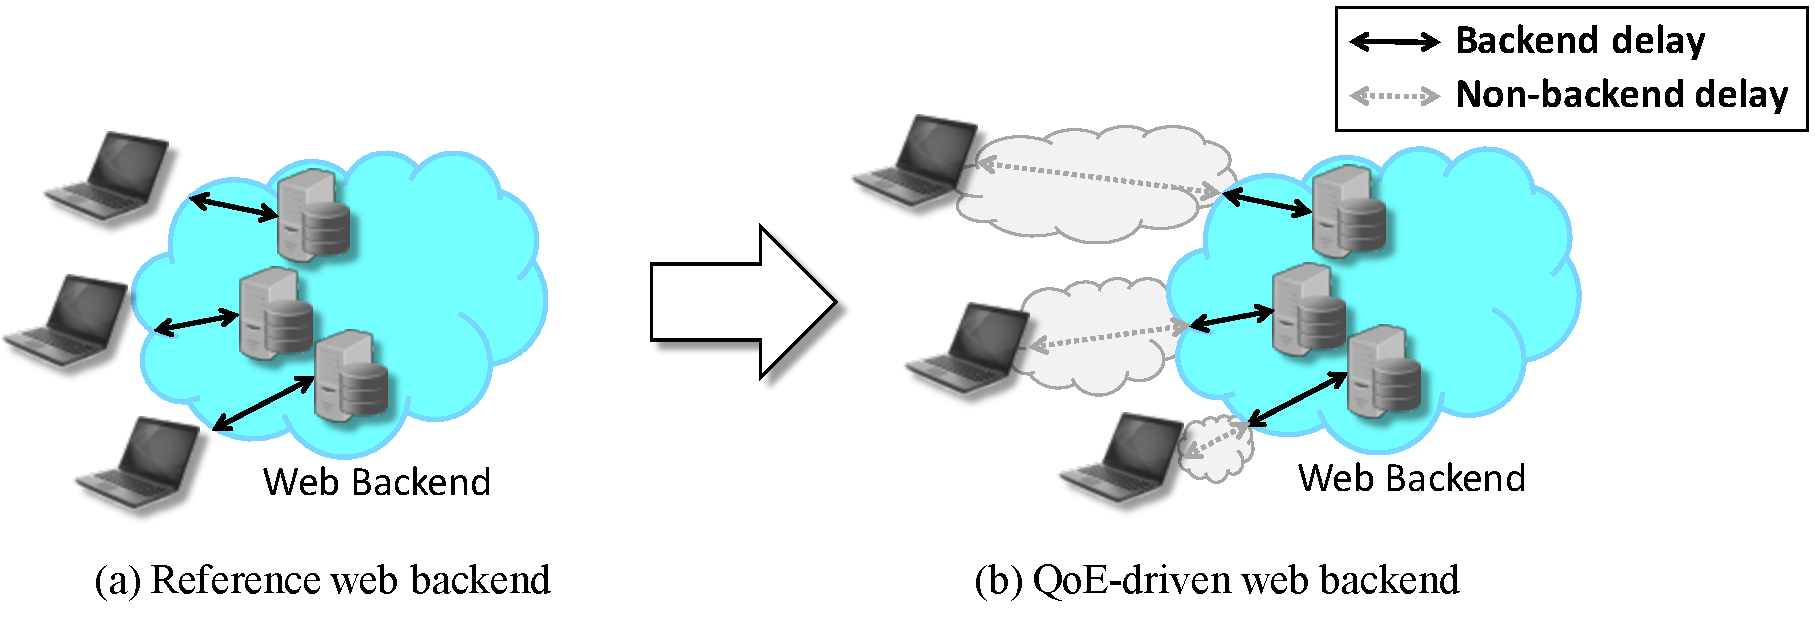
\includegraphics[width=0.9\textwidth]{figs/intro-overview.pdf}
	\vspace{-0.3cm}
	\caption{We propose to re-architect (a) the reference web backend which seeks to minimize the backend delays into (b) the QoE-driven web backend which seeks to minimize the impact of backend delay on user-perceived QoE.}
	\label{fig:intro-overview}
\end{figure}

%\jc{give a figure to contrast optimization of backend in-isolation vs. QoE-aware.}

%- Research goal: This project proposes that the web service backend should be aware of the QoE sensitivity. This effectively changes how one formulates the web service optimization problem.
\mypara{Research plan}
This proposal introduces ``QoE sensitivity'' as a new dimension for QoE optimization of web backends. 
Through developing novel algorithms and architectural components, we show that a {\bf QoE-driven web backend} (Figure~\ref{fig:intro-overview}(b)), which is aware of and exploits the differences of QoE sensitivity across requests, can substantially {\em improve the resource/QoE tradeoffs} of web service backend; \ie better QoE without using more resources, or saving resources without degrading QoE. 
% Note that being QoE sensitivity does not require expensive infrastructure changes (\eg adding hardware or changing software stack).
We divide the proposed research into four tasks.
%We use the following roadmap to thoroughly examine the benefits and challenges of QoE-sensitivity-aware web service backend.

\begin{packeditemize}
\item{\bf Quantifying potential benefits (Task \#1).}
We will design and carry out measurement studies to quantify the various improvements brought by QoE-driven web backend in the wild. We will provide a taxonomy of use cases of QoE-driven control in different aspects of today's web backend. We will also use large dataset from commercial web services to help understand opportunities in the actual traffic pattern in real world.

\item{\bf QoE-driven control algorithms (Task \#2).}
We will develop and build prototype of novel QoE-driven control policies for web backend, including resource allocation, message scheduling, and replica selection. Our design goals are (1) that the policies should balance near-optimal QoE and efficiency (minimal overhead of decision-making), and (2) that the implementation of these policies should be amenable to existing systems (\eg only control-plan changes).

\item{\bf QoE-driven backend architectural (Task \#3).}
We will develop new architectural component of web backend, including tracing infrastructure and QoE prediction models, to estimate the QoE sensitivity of requests in real-time. In the process, we will investigate the possibility of incremental deployment through reusing the existing tracing and telemetry infrastructure in large-scale web backends as much as possible.

\item{\bf Impact on QoE fairness (Task \#4).}
Finally, we will explore appropriate definitions of fairness to characterize the outcome of QoE-driven web backend. This would help us strike a desirable balance between QoE-driven optimization and QoE fairness. This would also help us recognize potential threads of other systems/users taking advantage of the QoE-driven policies of the backend.

\end{packeditemize}


%\jc{why these applications?}

%\jc{Common challenges! getting QoE sensitivity, fairness definition!}

\mypara{PI qualification}
The PI's expertise includes computer networking, Internet QoE, and data analytics systems.
He has published 11 peer-reviewed research papers (6 first-authored) in top-tier networking and system conferences (\ie SIGCOMM, NSDI, CoNEXT).
More importantly, the PI has a deep understanding of Internet QoE. His doctoral dissertation, titled ``Enabling Data-Driven Optimization of Quality of Experience in Internet Applications'', is among the first systematic studies to apply data-driven approach to improving Internet application QoE. The dissertation won the CMU SCS Doctoral Dissertation Award and was nominated for ACM Dissertation Award.
During his PhD and postdoctoral years, he has extensive collaborations with the industry, including Microsoft Research, Conviva Inc., and Google Research. These strong connections will help the proposed research to gain insights from the industry and provide viable path for deployment.


% \vspace{0.2cm}
% \noindent{\em Thrust \#1: How much potential benefit can we get?}

% \vspace{0.2cm}
% \noindent{\em Thrust \#2: How to re-architect web services to be QoE-aware?}

% \vspace{0.2cm}
% \noindent{\em Thrust \#3: How to propagate user-perceived QoE information?}

%- This project proposes to re-architect the web service backend by making it QoE-aware. Our roadmap has three steps.\\
%1. XXX\\
%2. YYY\\
%3. ZZZ



% \vspace{2cm}
% User-perceived quality of experience (QoE) is one of the driving forces behind the Internet ecosystem, which consists of {\em subsystems}, \eg datacenters, CDNs, cellular carriers, backbone networks, content providers, who share resources across users. 
% % End-to-end Quality of Experience (QoE) is the driving force behind today's Internet application ecosystem, which includes several subsystem
% % The Internet application ecosystem consists of many subsystems, Cloud, ISP, CDNs, etc, and 
% Thus, one fundamental question is {\em how to share resources across users in a way that optimizes their overall QoE?}
% The primary constraint is that these subsystems are {\em federated}: it is impractical to orchestrate a global optimization where they relinquish the control on how their resources are shared. 
% Instead, the conventional wisdom has been that each subsystem shares its resources among users in a way that optimizes the overall performance metrics within its limit and imposes no differentiation between users if they are ``functionally'' identical (\ie same service, business relationship, etc).

% In contrast, we are driven by a simple observation derived directly from the federated nature of the Internet ecosystem.
% In a subsystem, there is {\em a substantial heterogeneity} among its users with respect to how sensitive their QoE is to the performance of the subsystem, even if these users are functionally identical. 
% Thus, the right question to ask is {\em not} how a subsystem should optimize the overall performance among users; instead, it should minimize {\em overall impact on user-perceived QoE}, which requires treating users differently, rather than equally, depending on how much impact it has on the user's perceived QoE.

% In this proposal, we apply this idea to improving QoE of web services.

% \mypara{Research goals}

% \noindent {\bf Intellectual Merit.~~}
% This proposal applies this idea in the context of cloud services. 
% \jc{what it means to cloud services? requests are going to be treated differently, etc} 
% Specifically, this idea can be applied to many services inside a cloud. \jc{talk about more applications}
% In this project, we plan to answer three key question:

% First, how much potential benefit does this idea have?

% Second, how to design a QoE-aware cloud scheduling/resource allocation mechanism?

% Third, how to propogate QoE information from users to the cloud?

% \noindent {\bf Broader Impacts.~~}


% \noindent {\bf Keywords.~~} 



% QoE matters to everyone!

% \subsection{Missed Opportunities}
% \begin{itemize}

% \item Today's tenant: every user should be treated with the same performance goal. Implicit assumption is that the impact of a subsystem is the same on all users.

% \item However, the federated architecture means:\\
% 1. QoE can be affected by any subsystem\\
% 2. Each subsystem serves users with different QoE sensitivities.

% \item Fundamental mismatch: some users who are less sensitive to the subsystem get over-optimized, while others who are more sensitive to the subsystem get under-optimized.

% \item New approach: minimize the overall impact on QoE. 

% \end{itemize}

% \subsection{This proposal: Making Cloud QoE-Aware}
% \begin{itemize}

% \item How the cloud works today -- agnostic to QoE

% \item QoE curve

% \item Examples of how things can be done differently!

% \end{itemize}


% \subsection{Research Roadmap:}
% \begin{itemize}

% \item How much potential benefit does this idea have?

% \item How to design a QoE-aware cloud scheduling/resource allocation mechanism?

% \item How to propagate QoE information from users to the cloud?

% \end{itemize}

%
%\input{research}
%
%%% \input{example}
%
%%\input{example_junchen}
%
%\input{approach}
%
%\input{plan}
%
%\input{broader}
%
%\input{prior}

\newpage
\pagenumbering{arabic}
\renewcommand{\thepage} {E--\arabic{page}}
%\input{collaboration}


\newpage
\pagenumbering{arabic}
\renewcommand{\thepage} {F--\arabic{page}}
%\input{NSFData}

%%%%%%%%%%%%%%%%%%%%%%%%%%%%%%%%%%%%%%%%
%% F - BIOGRAPHICAL SKETCHES
%% provided separately - see cv_nsf.tex
%\newpage
%\section{Biographical Sketches}
%\newpage
%
%\addtolength{\voffset}{1in}
%\addtolength{\hoffset}{1in}
%
%\includepdf[pages=1-2]{Bios/Chien-NSF-Bio-2016v2}
%
%%%\textbf{John Birge}
%\includepdf[pages=1-2]{Bios/jrb_nsf_Biosketch_2016}
%\newpage
%%%\textbf{Victor Zavala}
%\includepdf[pages=1-2]{Bios/zavala-nsfbio.pdf}
%\addtolength{\voffset}{-1in}
%\addtolength{\hoffset}{-1in}

%%%%%%%%%%%%%%%%%%%%%%%%%%%%%%%%%%%%%%%
%%
%(8.b) Results of Prior Support (2 pages per person). Provide
%information only for the PI(s), each co-PI, and senior personnel, for
%contributions to research and education in science and engineering
%over the past five years (from any funding source). Include a brief
%statement of results of funded projects.


%%%%%%%%%%%%%%%%%%%%%%%%%%%%%%%%%%%%%%%
% E - REFERENCES CITED

\newpage
\pagenumbering{arabic}
\renewcommand{\thepage} {E--\arabic{page}}

\bibliographystyle{abbrv}
\bibliography{jiang,crii-qoe}

%\newpage

\addtolength{\voffset}{1in}
\addtolength{\hoffset}{1in}

%% \subsection{Andrew Chien}
%\includepdf[pages=1-2]{Bios/chien-prior.pdf}

%% \subsection{Hank Hoffmann}

%%\subsection{Junchen Jiang}}

%%%%%%%%%%%%%%%%%%%%%%%%%%%%%%%%%%%%%%%
%%
%% conflicts
\addtolength{\voffset}{-1in}
\addtolength{\hoffset}{-1in}


%%%%%%%%%%%%%%%%%%%%%%%%%%%%%%%%%%%%%%%
% H - CURRENT AND PENDING SUPPORT
% provided separately - see cv_nsf.tex
%% \newpage
%% \pagenumbering{arabic}

%% \renewcommand{\thepage} {F--\arabic{page}}

%% \newpage
%% \includepdf[page=1-2]{Admin/Chien-CP}

%%%%%%%%%%%%%%%%%%%%%%%%%%%%%%%%%%%%%%%
% G - BUDGET JUSTIFICATION

%% \newpage
%% \pagenumbering{arabic}
%% \renewcommand{\thepage} {G--\arabic{page}}
%% ~
%%\noindent{\Large \bf BUDGET JUSTIFICATION}

%% \includepdf[]{Admin/Chien-Budget-Just}

%%%%%%%%%%%%%%%%%%%%%%%%%%%%%%%%%%%%%%%
% H - DATA MANAGEMENT PLAN


%%  \addtolength{\voffset}{1in}
%%  \addtolength{\hoffset}{1in}

%% \newpage
%% \pagenumbering{arabic}
%% \setcounter{page}{1}
%% \renewcommand{\thepage} {H--\arabic{page}}
%% ~

%% \addtolength{\voffset}{-1in}
%% \addtolength{\hoffset}{-1in}

%\newpage
% \include{nsfdataman}
%\newpage

%%%%%%%%%%%%%%%%%%%%%%%%%%%%%%%%%%%%%%%
% I - FACILITIES & RESOURCES

%% \newpage
%% \pagenumbering{arabic}
%% \renewcommand{\thepage} {I--\arabic{page}}
%% %%\noindent{\Large \bf FACILITIES, EQUIPMENT, AND OTHER RESOURCES}\\

%\newpage
% \include{facilities}
%\newpage

%% \addtolength{\voffset}{1in}
%% \addtolength{\hoffset}{1in}

%% \includepdf[page=1-2]{Admin/Chien-Facilities}


%% \addtolength{\voffset}{-1in}
%% \addtolength{\hoffset}{-1in}

\end{document}
